\newpage
\section{ম্যাট্রিক্স এর সংজ্ঞা (Definition of Matrix)}
\begin{tcolorbox}[colback=green!5!white,colframe=green!75!black,title=\textbf{সংজ্ঞা}]
	নির্দিষ্ট সংখ্যক সংখ্যা, প্রতীক বা রাশি এর আয়তাকার বিন্যাসকে ম্যাট্রিক্স (Matrix) বলে।
\end{tcolorbox}
Example: 
$
A=[a_{ij}]=\begin{blockarray}{cccccc}
	\text{ ১ম কলাম} & \text{২য় কলাম} & \cdots & n\text{-তম কলাম} & &\\
	\pmb{\downarrow} & \pmb{\downarrow} & \cdots & \pmb{\downarrow} & & \\
	\begin{block}{[cccc]cc}
		a_{11} & a_{12} & \cdots & a_{1 n} & \pmb{\rightarrow} &\text{ ১ম সারি}\\ 
		a_{21} & a_{22} & \cdots & a_{2 n} & \pmb{\rightarrow} & \text{২য় সারি}\\
		\vdots & \vdots & \vdots & \vdots & & \vdots \\
		a_{m 1} & a_{m 2} & \cdots & a_{m n} & \pmb{\rightarrow} & m\text{-তম সারি}\\
	\end{block}
\end{blockarray}
$
যেখানে, সারি $i=1,2,\cdots,m$ এবং কলাম $j=1,2,\cdots,n$\\
একটি $m\times n$ (সারি সংখ্যা by কলাম সংখ্যা) আকারের ম্যাট্রিক্স।\\
ম্যাট্রিক্স বোঝাতে $[\hspace{8pt}], (\hspace{8pt})$ বা $\left|\right|\hspace{4pt}\left|\right|$ ব্যবহার করা হয়।
\begin{tcolorbox}
	\begin{itemize}
		\item[$\bullet$] \textbf{ভুক্তি (Entry):} ম্যাট্রিক্স অন্তর্গত সংখ্যাগুলিকে ভুক্তি (Entry) বলে। $a_{ij}$ হলো $(i,j)$ -তম ভুক্তি যেখানে $i=$ সারি নাম্বার এবং $j=$ কলাম নাম্বার। 
		\item[$\bullet$] \textbf{ক্রম (Order):} কোন ম্যাট্রিক্স এর সারির সংখ্যা $m$ ও কলাম সংখ্যা $n$ হলে $m \times n$ কে ঐ ম্যাট্রিক্স এর ক্রম (Order) বলে।
	\end{itemize}
\end{tcolorbox}
\begin{figure}[h]
	\centering
	

\tikzset{every picture/.style={line width=0.75pt}} %set default line width to 0.75pt        

\begin{tikzpicture}[x=0.75pt,y=0.75pt,yscale=-1,xscale=1]
%uncomment if require: \path (0,300); %set diagram left start at 0, and has height of 300

%Straight Lines [id:da586819984425849] 
\draw    (120,70) -- (120,214) ;
%Straight Lines [id:da7562437314920758] 
\draw    (120,70) -- (136.11,70) ;
%Straight Lines [id:da07321515917820864] 
\draw    (120,214) -- (136.11,214) ;

%Straight Lines [id:da5879432373101097] 
\draw    (345.56,214) -- (345.56,70) ;
%Straight Lines [id:da032030890290525305] 
\draw    (345.56,214) -- (329.44,214) ;
%Straight Lines [id:da356184097761693] 
\draw    (345.56,70) -- (329.44,70) ;

%Straight Lines [id:da5886141084026595] 
\draw    (410,215) -- (457.54,181.72) ;
\draw [shift={(460,180)}, rotate = 505.01] [fill={rgb, 255:red, 0; green, 0; blue, 0 }  ][line width=0.08]  [draw opacity=0] (10.72,-5.15) -- (0,0) -- (10.72,5.15) -- (7.12,0) -- cycle    ;
%Shape: Brace [id:dp5361591699619341] 
\draw   (82.5,76) .. controls (77.83,76) and (75.5,78.33) .. (75.5,83) -- (75.5,133.5) .. controls (75.5,140.17) and (73.17,143.5) .. (68.5,143.5) .. controls (73.17,143.5) and (75.5,146.83) .. (75.5,153.5)(75.5,150.5) -- (75.5,204) .. controls (75.5,208.67) and (77.83,211) .. (82.5,211) ;
%Shape: Brace [id:dp38183115425296243] 
\draw   (330.5,59) .. controls (330.53,54.33) and (328.21,51.99) .. (323.54,51.96) -- (243.04,51.56) .. controls (236.37,51.53) and (233.05,49.18) .. (233.07,44.51) .. controls (233.05,49.18) and (229.71,51.49) .. (223.04,51.46)(226.04,51.47) -- (142.54,51.05) .. controls (137.87,51.02) and (135.53,53.34) .. (135.5,58.01) ;
%Shape: Ellipse [id:dp6713629060951722] 
\draw   (350,215) .. controls (350,206.72) and (363.43,200) .. (380,200) .. controls (396.57,200) and (410,206.72) .. (410,215) .. controls (410,223.28) and (396.57,230) .. (380,230) .. controls (363.43,230) and (350,223.28) .. (350,215) -- cycle ;
%Shape: Circle [id:dp32711506861948525] 
\draw   (238.69,140.1) .. controls (239.41,129) and (249,120.59) .. (260.1,121.31) .. controls (271.21,122.03) and (279.62,131.62) .. (278.9,142.72) .. controls (278.18,153.82) and (268.59,162.24) .. (257.49,161.52) .. controls (246.39,160.79) and (237.97,151.21) .. (238.69,140.1) -- cycle ;
%Curve Lines [id:da8891858202718295] 
\draw    (260.1,121.31) .. controls (299.11,43.78) and (363.2,54.77) .. (408.63,88.96) ;
\draw [shift={(410,90)}, rotate = 217.57] [color={rgb, 255:red, 0; green, 0; blue, 0 }  ][line width=0.75]    (10.93,-3.29) .. controls (6.95,-1.4) and (3.31,-0.3) .. (0,0) .. controls (3.31,0.3) and (6.95,1.4) .. (10.93,3.29)   ;
%Straight Lines [id:da3652967556576887] 
\draw    (360,230) -- (331.9,239.37) ;
\draw [shift={(330,240)}, rotate = 341.57] [color={rgb, 255:red, 0; green, 0; blue, 0 }  ][line width=0.75]    (10.93,-3.29) .. controls (6.95,-1.4) and (3.31,-0.3) .. (0,0) .. controls (3.31,0.3) and (6.95,1.4) .. (10.93,3.29)   ;
%Straight Lines [id:da660228436313117] 
\draw    (400,230) -- (438.06,239.51) ;
\draw [shift={(440,240)}, rotate = 194.04] [color={rgb, 255:red, 0; green, 0; blue, 0 }  ][line width=0.75]    (10.93,-3.29) .. controls (6.95,-1.4) and (3.31,-0.3) .. (0,0) .. controls (3.31,0.3) and (6.95,1.4) .. (10.93,3.29)   ;

% Text Node
\draw (151.54,79.95) node [anchor=north west][inner sep=0.75pt]    {$1$};
% Text Node
\draw (203.2,79.95) node [anchor=north west][inner sep=0.75pt]    {$2$};
% Text Node
\draw (254.86,79.95) node [anchor=north west][inner sep=0.75pt]    {$3$};
% Text Node
\draw (151.54,135.4) node [anchor=north west][inner sep=0.75pt]    {$5$};
% Text Node
\draw (203.2,135.4) node [anchor=north west][inner sep=0.75pt]    {$6$};
% Text Node
\draw (254.86,135.4) node [anchor=north west][inner sep=0.75pt]    {$7$};
% Text Node
\draw (151.54,190.85) node [anchor=north west][inner sep=0.75pt]    {$9$};
% Text Node
\draw (195.39,190.85) node [anchor=north west][inner sep=0.75pt]    {$10$};
% Text Node
\draw (247.05,190.85) node [anchor=north west][inner sep=0.75pt]    {$11$};
% Text Node
\draw (306.52,79.95) node [anchor=north west][inner sep=0.75pt]    {$4$};
% Text Node
\draw (306.52,135.4) node [anchor=north west][inner sep=0.75pt]    {$8$};
% Text Node
\draw (298.71,190.85) node [anchor=north west][inner sep=0.75pt]    {$12$};
% Text Node
\draw (360.08,206.4) node [anchor=north west][inner sep=0.75pt]    {$3\times 4$};
% Text Node
\draw (1,141) node [anchor=north west][inner sep=0.75pt]   [align=left] {$3$ টি সারি};
% Text Node
\draw (201,22) node [anchor=north west][inner sep=0.75pt]   [align=left] {$4$ টি কলাম};
% Text Node
\draw (431,152) node [anchor=north west][inner sep=0.75pt]   [align=left] {ম্যাট্রিক্স এর ক্রম };
% Text Node
\draw (281,241) node [anchor=north west][inner sep=0.75pt]   [align=left] {সারি সংখ্যা};
% Text Node
\draw (448,232) node [anchor=north west][inner sep=0.75pt]   [align=left] {কলাম সংখ্যা};
% Text Node
\draw (409,82.4) node [anchor=north west][inner sep=0.75pt]    {$(2,3)$তম ভুক্তি $=a_{23}$};
% Text Node
\draw (83,132.4) node [anchor=north west][inner sep=0.75pt]    {$A=$};


\end{tikzpicture}
	\caption{একটি ম্যাট্রিক্স}
	\label{mat-fig-1}
\end{figure}
\section{ম্যাট্রিক্স এর প্রকারভেদ (Classification of Matrix)}
\begin{enumerate}
	\item \textbf{আয়তাকার ম্যাট্রিক্স (Rectangular Matrix):} যদি কোনো $m \times n$ আকারের ম্যাট্রিক্স এ $m\neq n$ হয় তবে তাকে আয়তাকার ম্যাট্রিক্স বলে। Example: 
	$\left[\begin{array}{rrr}
		2 & -1 & 3 \\
		3 & 6 & -4
	\end{array}\right]$ একটি $2 \times 3$ আকারের আয়তাকার ম্যাট্রিক্স।
	
	\item \textbf{সারি ম্যাট্রিক্স (Row Matrix):} কেবল একটি সারি সম্বলিত ম্যাট্রিক্স কে সারি মাত্রিক্সক বলে। Example: 
	$\left[\begin{array}{ccc}
	11 & 12 & 13
	\end{array}\right]_{1 \times 3}$ একটি $1 \times 3$ ক্রমের সারি ম্যাট্রিক্স।
	
	\item \textbf{কলাম ম্যাট্রিক্স (Column Matrix):} কেবল একটি কলাম সম্বলিত ম্যাট্রিক্স কে কলাম ম্যাট্রিক্স বলে। Example: 
	$\left[\begin{array}{c}
	11 \\ 12 \\ 13
	\end{array}\right]_{3 \times 1}$ একটি $3 \times 1$ আকারের কলাম ম্যাট্রিক্স।
	
	\item \textbf{বর্গ ম্যাট্রিক্স (Square Matrix):} কোনো ম্যাট্রিক্স এর সারি ও কলাম সংখ্যা সমান $(m=n)$ হলে তাকে বর্গ ম্যাট্রিক্স বলে। Example: 
	$
	\left[\begin{array}{ccc}
	2 & 4 & 5 \\
	5 & 6 & 8 \\
	4 & 5 & 6
	\end{array}\right]_{3 \times 3}
	$ একটি $3\times3$ বর্গ ম্যাট্রিক্স।\\ 
	\begin{tcolorbox}
		\begin{itemize}
			\item[$\bullet$] \textbf{মুখ্যকর্ণ (Principal Diagonal):} ম্যাট্রিক্স $(1,1)$-তম ভুক্তিগামি কর্ণকে মুখ্যকর্ণ বলে। Example: 
			$
			\left[\begin{array}{ccc}
			\textcolor{red}{1} & 0 & 0 \\
			0 & \textcolor{red}{1} & 0 \\
			0 & 0 & \textcolor{red}{1}
			\end{array}\right], 
			\left[\begin{array}{cccc}
			\textcolor{red}{1} & 0 & 0 & 0 \\
			0 & \textcolor{red}{1} & 0 & 0 \\
			0 & 0 & \textcolor{red}{1} & 0
			\end{array}\right]
			$
			\item[$\bullet$] \textbf{গৌণকর্ণ (Anti-diagonal):} কোনো $m\times m$ ক্রমের বর্গ ম্যাট্রিক্স এর $(1,m)$ বা $(m,1)$-তম ভুক্তিগামি কর্ণকে গৌণকর্ণ বলে।\\ Example: 
			$
			\left[\begin{array}{ccc}
			0 & 0 & \textcolor{red}{1} \\
			0 & \textcolor{red}{1} & 0 \\
			\textcolor{red}{1} & 0 & 0
			\end{array}\right]
			$\\
			\item[$\bullet$] \textbf{ট্রেস (Trace):} কোনো বর্গ ম্যাট্রিক্স এর মুখ্যকর্ণের ভুক্তিগুলোর সমষ্টিকে ট্রেস বলে।\\ Example:
			$
			\left[\begin{array}{ccc}
			\textcolor{red}{a_{11}} & a_{12} & a_{13} \\
			a_{21} & \textcolor{red}{a_{22}} & a_{23} \\
			a_{31} & a_{32} & \textcolor{red}{a_{33}}
			\end{array}\right]
			$ ম্যাট্রিক্সটির ট্রেস$=\textcolor{red}{a_{11}+a_{22}+a_{33}}$\\
		\end{itemize}
	\end{tcolorbox}
	\item \textbf{কর্ণ ম্যাট্রিক্স (Diagonal Matrix):} যে বর্গ ম্যাট্রিক্স এর মুখ্যকর্ণের ভুক্তিগুলো ব্যতীত বাকি সকল ভুক্তিগুলো শূন্য তাকে কর্ণ ম্যাট্রিক্স বলে। \\
	Example:
	$\left[\begin{array}{ccc}
	a & 0 & 0 \\
	0 & b & 0 \\
	0 & 0 & c
	\end{array}\right]$ একটি কর্ণ ম্যাট্রিক্স যেখানে $a\neq b\neq c\neq 0$। 
	 
	\item \textbf{স্কেলার ম্যাট্রিক্স (Scalar Matrix):} কর্ণ ম্যাট্রিক্স এর অশূন্য ভুক্তিগুলো সমান হলে তাকে স্কেলার ম্যাট্রিক্স বলে। \\
	Example: 
	$\left[\begin{array}{ccc}
	k & 0 & 0 \\
	0 & k & 0 \\
	0 & 0 & k
	\end{array}\right]$ একটি কর্ণ ম্যাট্রিক্স যেখানে $k\neq 0$।
	\item \textbf{অভেদক ম্যাট্রিক্স (Identity Matrix):} স্কেলার ম্যাট্রিক্স এর অশূন্য ভুক্তিগুলোর মান $1$ হলে তাকে অভেদক ম্যাট্রিক্স বলে। একে $I_{n}$ দ্বারা প্রকাশ করা হয়।\\ Example: 
	$
	I_{n}=\left[\begin{array}{cccc}
	1 & 0 & \cdots & 0 \\
	0 & 1 & \cdots & 0 \\
	\cdots & \cdots & \cdots & \cdots\\
	0 & 0 & \cdots & 1 
	\end{array}\right],
	I_{2}=\left[\begin{array}{cc}
	1 & 0 \\
	0 & 1
	\end{array}\right],
	I_{3}=\left[\begin{array}{ccc}
	1 & 0 & 0\\
	0 & 1 & 0\\
	0 & 0 & 1
	\end{array}\right]
	$।
	
	\item \textbf{শূন্য ম্যাট্রিক্স (Null Matrix):} যে ম্যাট্রিক্স এর সকল ভুক্তি শূন্য তাকে শূন্য ম্যাট্রিক্স বলে। Example: 
	$\left[\begin{array}{cc}
	0 & 0 \\
	0 & 0
	\end{array}\right], 
	\left[\begin{array}{ccc}
	0 & 0 & 0\\
	0 & 0 & 0\\
	0 & 0 & 0
	\end{array}\right]$।
	
	\item \textbf{ত্রিভুজাকার ম্যাট্রিক্স (Triangular Matrix):} যে বর্গ ম্যাট্রিক্স এর মুখ্য কর্ণের নিচে বা উপরের ভুক্তিগুলো শূন্য তাকে ত্রিভুজাকার ম্যাট্রিক্স বলে।\\ Example: 
	$
	\left[\begin{array}{ccc}
	\textcolor{red}{2} & 0 & 0 \\
	\textcolor{red}{6} & \textcolor{red}{9} & 0 \\
	\textcolor{red}{9} & \textcolor{red}{6} & \textcolor{red}{6}
	\end{array}\right], 
	\left[\begin{array}{ccc}
	\textcolor{red}{2} & \textcolor{red}{1} & \textcolor{red}{6} \\
	0 & \textcolor{red}{9} & \textcolor{red}{5} \\
	0 & 0 & \textcolor{red}{3}
	\end{array}\right]
	$।
	\begin{tcolorbox}
		\begin{itemize}
			\item[$\bullet$] \textbf{ ঊর্ধ্ব ত্রিভুজাকার ম্যাট্রিক্স (Upper Triangular Matrix):} বর্গ ম্যাট্রিক্স এর মুখ্য কর্ণের নিচের সকল ভুক্তি শূন্য।\\ Example: 
			$A=[a_{ij}]=
			\left[\begin{array}{ccc}
			\textcolor{red}{2} & \textcolor{red}{1} & \textcolor{red}{6} \\
			0 & \textcolor{red}{9} & \textcolor{red}{5} \\
			0 & 0 & \textcolor{red}{3}
			\end{array}\right]$ যেখানে $a_{ij}=0$ এবং $i>j$। 
			\item[$\bullet$] \textbf{ নিম্ন ত্রিভুজাকার ম্যাট্রিক্স (Lower Triangular Matrix):} বর্গ ম্যাট্রিক্স এর মুখ্য কর্ণের উপরের সকল ভুক্তি শূন্য।\\ Example: 
			$A=[a_{ij}]=\left[\begin{array}{ccc}
			\textcolor{red}{2} & 0 & 0 \\
			\textcolor{red}{6} & \textcolor{red}{9} & 0 \\
			\textcolor{red}{9} & \textcolor{red}{6} & \textcolor{red}{6}
			\end{array}\right]$ যেখানে $a_{ij}=0$ এবং $i<j$। 
		\end{itemize}
	\end{tcolorbox}

	\item \textbf{বিম্ব ম্যাট্রিক্স (Transpose Matrix):} কোনো ম্যাট্রিক্স $A$ এর কলামগুলোকে সারি এবং সারিগুলোকে কলাম এ পরিনত করলে যে ম্যাট্রিক্স পাওয়া যায় তাকে ঐ ম্যাট্রিক্স এর বিম্ব ম্যাট্রিক্স বলে যাকে $A^T$ দ্বারা প্রকাশ করা হয়।\\ Example: 
	$A=\left[\begin{array}{ccc}
	2 & 5 & 8 \\
	6 & 9 & 0 \\
	9 & 6 & 6
	\end{array}\right]$ হলে 
	$A^T=\left[\begin{array}{ccc}
	2 & 6 & 9 \\
	5 & 9 & 6 \\
	8 & 0 & 6
	\end{array}\right]$।
	\begin{figure}[h]
		\centering
		

\tikzset{every picture/.style={line width=0.75pt}} %set default line width to 0.75pt        

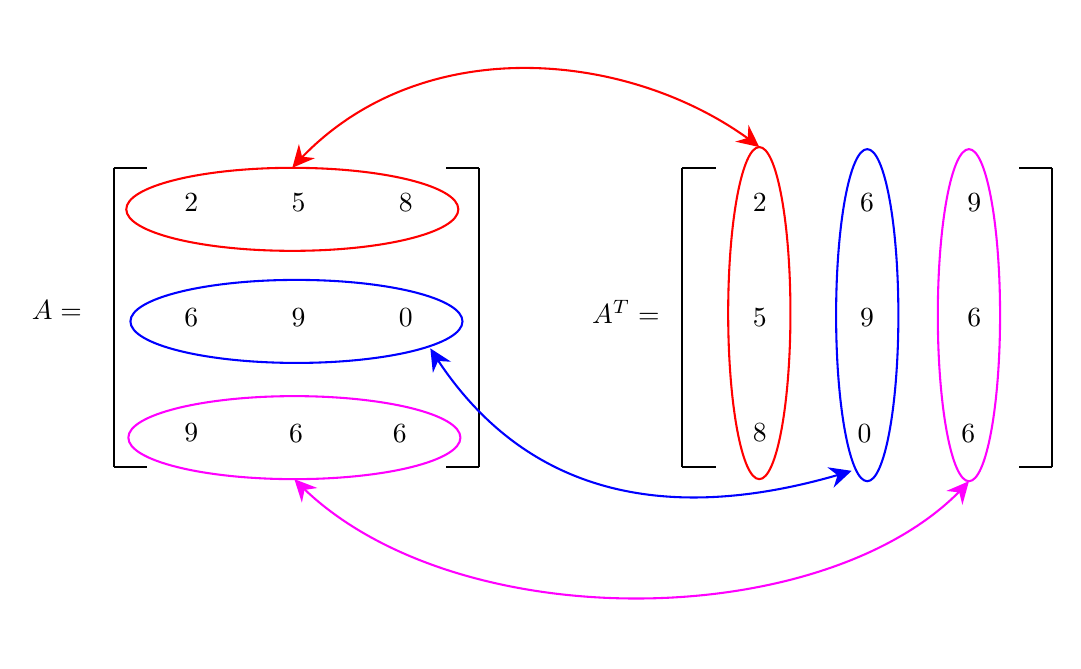
\begin{tikzpicture}[x=0.75pt,y=0.75pt,yscale=-1,xscale=1]
%uncomment if require: \path (0,300); %set diagram left start at 0, and has height of 300

%Straight Lines [id:da2213819570252611] 
\draw    (93.89,70) -- (93.89,214) ;
%Straight Lines [id:da29721507169372896] 
\draw    (93.89,70) -- (110,70) ;
%Straight Lines [id:da35934426602025504] 
\draw    (93.89,214) -- (110,214) ;

%Straight Lines [id:da6023748561134159] 
\draw    (270,214) -- (270,70) ;
%Straight Lines [id:da4805786206905196] 
\draw    (270,214) -- (253.89,214) ;
%Straight Lines [id:da5967411370774598] 
\draw    (270,70) -- (253.89,70) ;

%Straight Lines [id:da9049186085059904] 
\draw    (367.78,70) -- (367.78,214) ;
%Straight Lines [id:da6931297695132848] 
\draw    (367.78,70) -- (383.89,70) ;
%Straight Lines [id:da7325439366388315] 
\draw    (367.78,214) -- (383.89,214) ;

%Straight Lines [id:da9297150199392166] 
\draw    (546.11,214) -- (546.11,70) ;
%Straight Lines [id:da17597738471086588] 
\draw    (546.11,214) -- (530,214) ;
%Straight Lines [id:da9212767075909833] 
\draw    (546.11,70) -- (530,70) ;

%Shape: Ellipse [id:dp6011237777220346] 
\draw  [color={rgb, 255:red, 255; green, 0; blue, 0 }  ,draw opacity=1 ] (100,90) .. controls (100,78.95) and (135.82,70) .. (180,70) .. controls (224.18,70) and (260,78.95) .. (260,90) .. controls (260,101.05) and (224.18,110) .. (180,110) .. controls (135.82,110) and (100,101.05) .. (100,90) -- cycle ;
%Shape: Ellipse [id:dp9649907352391565] 
\draw  [color={rgb, 255:red, 255; green, 0; blue, 0 }  ,draw opacity=1 ] (405,60) .. controls (413.28,60) and (420,95.82) .. (420,140) .. controls (420,184.18) and (413.28,220) .. (405,220) .. controls (396.72,220) and (390,184.18) .. (390,140) .. controls (390,95.82) and (396.72,60) .. (405,60) -- cycle ;
%Shape: Ellipse [id:dp49968264093049886] 
\draw  [color={rgb, 255:red, 0; green, 0; blue, 255 }  ,draw opacity=1 ] (102,144) .. controls (102,132.95) and (137.82,124) .. (182,124) .. controls (226.18,124) and (262,132.95) .. (262,144) .. controls (262,155.05) and (226.18,164) .. (182,164) .. controls (137.82,164) and (102,155.05) .. (102,144) -- cycle ;
%Shape: Ellipse [id:dp12864677020337312] 
\draw  [color={rgb, 255:red, 255; green, 0; blue, 255 }  ,draw opacity=1 ] (101,200) .. controls (101,188.95) and (136.82,180) .. (181,180) .. controls (225.18,180) and (261,188.95) .. (261,200) .. controls (261,211.05) and (225.18,220) .. (181,220) .. controls (136.82,220) and (101,211.05) .. (101,200) -- cycle ;
%Shape: Ellipse [id:dp02487303364640492] 
\draw  [color={rgb, 255:red, 0; green, 0; blue, 255 }  ,draw opacity=1 ] (457,61) .. controls (465.28,61) and (472,96.82) .. (472,141) .. controls (472,185.18) and (465.28,221) .. (457,221) .. controls (448.72,221) and (442,185.18) .. (442,141) .. controls (442,96.82) and (448.72,61) .. (457,61) -- cycle ;
%Shape: Ellipse [id:dp312374845137267] 
\draw  [color={rgb, 255:red, 255; green, 0; blue, 255 }  ,draw opacity=1 ] (506,61) .. controls (514.28,61) and (521,96.82) .. (521,141) .. controls (521,185.18) and (514.28,221) .. (506,221) .. controls (497.72,221) and (491,185.18) .. (491,141) .. controls (491,96.82) and (497.72,61) .. (506,61) -- cycle ;
%Curve Lines [id:da9481816921410489] 
\draw [color={rgb, 255:red, 255; green, 0; blue, 0 }  ,draw opacity=1 ]   (182.71,66.99) .. controls (242.07,2.98) and (344.32,13.49) .. (403.23,58.62) ;
\draw [shift={(405,60)}, rotate = 218.31] [fill={rgb, 255:red, 255; green, 0; blue, 0 }  ,fill opacity=1 ][line width=0.08]  [draw opacity=0] (10.72,-5.15) -- (0,0) -- (10.72,5.15) -- (7.12,0) -- cycle    ;
\draw [shift={(180,70)}, rotate = 311.19] [fill={rgb, 255:red, 255; green, 0; blue, 0 }  ,fill opacity=1 ][line width=0.08]  [draw opacity=0] (10.72,-5.15) -- (0,0) -- (10.72,5.15) -- (7.12,0) -- cycle    ;
%Curve Lines [id:da7276678073856719] 
\draw [color={rgb, 255:red, 0; green, 0; blue, 255 }  ,draw opacity=1 ]   (248.45,160.11) .. controls (291.17,226.83) and (359.47,243.25) .. (446.85,216.81) ;
\draw [shift={(449.5,216)}, rotate = 522.72] [fill={rgb, 255:red, 0; green, 0; blue, 255 }  ,fill opacity=1 ][line width=0.08]  [draw opacity=0] (10.72,-5.15) -- (0,0) -- (10.72,5.15) -- (7.12,0) -- cycle    ;
\draw [shift={(246.5,157)}, rotate = 58.44] [fill={rgb, 255:red, 0; green, 0; blue, 255 }  ,fill opacity=1 ][line width=0.08]  [draw opacity=0] (10.72,-5.15) -- (0,0) -- (10.72,5.15) -- (7.12,0) -- cycle    ;
%Curve Lines [id:da16259241119309786] 
\draw [color={rgb, 255:red, 255; green, 0; blue, 255 }  ,draw opacity=1 ]   (183.24,222.32) .. controls (257.48,297.18) and (438.48,294.33) .. (504.05,223.18) ;
\draw [shift={(506,221)}, rotate = 491.08] [fill={rgb, 255:red, 255; green, 0; blue, 255 }  ,fill opacity=1 ][line width=0.08]  [draw opacity=0] (10.72,-5.15) -- (0,0) -- (10.72,5.15) -- (7.12,0) -- cycle    ;
\draw [shift={(181,220)}, rotate = 46.7] [fill={rgb, 255:red, 255; green, 0; blue, 255 }  ,fill opacity=1 ][line width=0.08]  [draw opacity=0] (10.72,-5.15) -- (0,0) -- (10.72,5.15) -- (7.12,0) -- cycle    ;

% Text Node
\draw (126.54,80.95) node [anchor=north west][inner sep=0.75pt]    {$2$};
% Text Node
\draw (178.2,80.95) node [anchor=north west][inner sep=0.75pt]    {$5$};
% Text Node
\draw (229.86,80.95) node [anchor=north west][inner sep=0.75pt]    {$8$};
% Text Node
\draw (126.54,136.4) node [anchor=north west][inner sep=0.75pt]    {$6$};
% Text Node
\draw (178.2,136.4) node [anchor=north west][inner sep=0.75pt]    {$9$};
% Text Node
\draw (229.86,136.4) node [anchor=north west][inner sep=0.75pt]    {$0$};
% Text Node
\draw (126.54,191.85) node [anchor=north west][inner sep=0.75pt]    {$9$};
% Text Node
\draw (177,192.4) node [anchor=north west][inner sep=0.75pt]    {$6$};
% Text Node
\draw (227,192.4) node [anchor=north west][inner sep=0.75pt]    {$6$};
% Text Node
\draw (53,132.4) node [anchor=north west][inner sep=0.75pt]    {$A=$};
% Text Node
\draw (400.43,80.95) node [anchor=north west][inner sep=0.75pt]    {$2$};
% Text Node
\draw (452.09,80.95) node [anchor=north west][inner sep=0.75pt]    {$6$};
% Text Node
\draw (503.75,80.95) node [anchor=north west][inner sep=0.75pt]    {$9$};
% Text Node
\draw (400.43,136.4) node [anchor=north west][inner sep=0.75pt]    {$5$};
% Text Node
\draw (452.09,136.4) node [anchor=north west][inner sep=0.75pt]    {$9$};
% Text Node
\draw (503.75,136.4) node [anchor=north west][inner sep=0.75pt]    {$6$};
% Text Node
\draw (400.43,191.85) node [anchor=north west][inner sep=0.75pt]    {$8$};
% Text Node
\draw (450.89,192.4) node [anchor=north west][inner sep=0.75pt]    {$0$};
% Text Node
\draw (500.89,192.4) node [anchor=north west][inner sep=0.75pt]    {$6$};
% Text Node
\draw (323,132.4) node [anchor=north west][inner sep=0.75pt]    {$A^{T}=$};


\end{tikzpicture}
		\caption{বিম্ব ম্যাট্রিক্স}
		\label{mat-fig-2}
	\end{figure}
	
	\item \textbf{প্রতিসম ম্যাট্রিক্স (Symmetric Matrix):} কোনো বর্গ ম্যাট্রিক্স $A=[a_{ij}]$ এবং এর ট্রান্সপজ ম্যাট্রিক্স পরস্পর সমান হলে অর্থাৎ $a_{ij}=a_{ji}$ তাকে প্রতিসম ম্যাট্রিক্স বলা হয়।\\ Example: 
	$A=\left[\begin{array}{rrr}
	5 & 2 & 1 \\
	2 & 6 & -1 \\
	1 & -1 & 4
	\end{array}\right]
	$ হলে 
	$A^T=\left[\begin{array}{rrr}
	5 & 2 & 1 \\
	2 & 6 & -1 \\
	1 & -1 & 4
	\end{array}\right]$ এখানে $A=A^T$। সুতরাং $A$ একটি প্রতিসম ম্যাট্রিক্স।
	\begin{figure}[h]
		\centering
		

\tikzset{every picture/.style={line width=0.75pt}} %set default line width to 0.75pt        

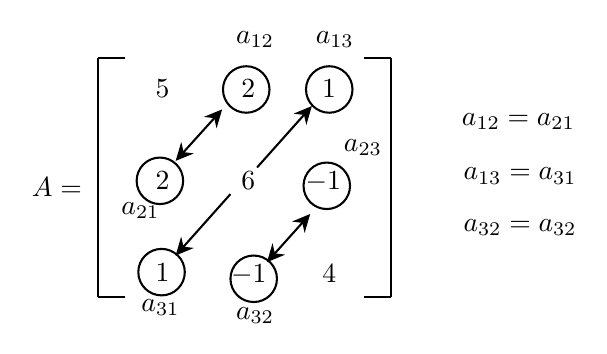
\begin{tikzpicture}[x=0.75pt,y=0.75pt,yscale=-0.8,xscale=0.8]
%uncomment if require: \path (0,300); %set diagram left start at 0, and has height of 300

%Straight Lines [id:da10936724554867983] 
\draw    (197.89,60) -- (197.89,204) ;
%Straight Lines [id:da05872790918592985] 
\draw    (197.89,60) -- (214,60) ;
%Straight Lines [id:da5439709419136995] 
\draw    (197.89,204) -- (214,204) ;

%Straight Lines [id:da3622304630394042] 
\draw    (374,204) -- (374,60) ;
%Straight Lines [id:da15386640282905906] 
\draw    (374,204) -- (357.89,204) ;
%Straight Lines [id:da9343614079600226] 
\draw    (374,60) -- (357.89,60) ;

%Straight Lines [id:da6043535743186701] 
\draw    (246.51,119.77) -- (270.49,93.23) ;
\draw [shift={(272.5,91)}, rotate = 492.09] [fill={rgb, 255:red, 0; green, 0; blue, 0 }  ][line width=0.08]  [draw opacity=0] (10.72,-5.15) -- (0,0) -- (10.72,5.15) -- (7.12,0) -- cycle    ;
\draw [shift={(244.5,122)}, rotate = 312.09] [fill={rgb, 255:red, 0; green, 0; blue, 0 }  ][line width=0.08]  [draw opacity=0] (10.72,-5.15) -- (0,0) -- (10.72,5.15) -- (7.12,0) -- cycle    ;
%Straight Lines [id:da4019864480926032] 
\draw    (301.5,180.77) -- (323.5,156.23) ;
\draw [shift={(325.5,154)}, rotate = 491.88] [fill={rgb, 255:red, 0; green, 0; blue, 0 }  ][line width=0.08]  [draw opacity=0] (10.72,-5.15) -- (0,0) -- (10.72,5.15) -- (7.12,0) -- cycle    ;
\draw [shift={(299.5,183)}, rotate = 311.88] [fill={rgb, 255:red, 0; green, 0; blue, 0 }  ][line width=0.08]  [draw opacity=0] (10.72,-5.15) -- (0,0) -- (10.72,5.15) -- (7.12,0) -- cycle    ;
%Shape: Circle [id:dp995842930403152] 
\draw   (273,79) .. controls (273,71.27) and (279.27,65) .. (287,65) .. controls (294.73,65) and (301,71.27) .. (301,79) .. controls (301,86.73) and (294.73,93) .. (287,93) .. controls (279.27,93) and (273,86.73) .. (273,79) -- cycle ;
%Shape: Circle [id:dp5704385344425422] 
\draw   (221,134) .. controls (221,126.27) and (227.27,120) .. (235,120) .. controls (242.73,120) and (249,126.27) .. (249,134) .. controls (249,141.73) and (242.73,148) .. (235,148) .. controls (227.27,148) and (221,141.73) .. (221,134) -- cycle ;
%Shape: Circle [id:dp2175701824695302] 
\draw   (323,79) .. controls (323,71.27) and (329.27,65) .. (337,65) .. controls (344.73,65) and (351,71.27) .. (351,79) .. controls (351,86.73) and (344.73,93) .. (337,93) .. controls (329.27,93) and (323,86.73) .. (323,79) -- cycle ;
%Shape: Circle [id:dp7718278958038063] 
\draw   (222,189) .. controls (222,181.27) and (228.27,175) .. (236,175) .. controls (243.73,175) and (250,181.27) .. (250,189) .. controls (250,196.73) and (243.73,203) .. (236,203) .. controls (228.27,203) and (222,196.73) .. (222,189) -- cycle ;
%Shape: Circle [id:dp7676418419992876] 
\draw   (321.5,137) .. controls (321.5,129.27) and (327.77,123) .. (335.5,123) .. controls (343.23,123) and (349.5,129.27) .. (349.5,137) .. controls (349.5,144.73) and (343.23,151) .. (335.5,151) .. controls (327.77,151) and (321.5,144.73) .. (321.5,137) -- cycle ;
%Shape: Circle [id:dp7454501087701606] 
\draw   (277.5,193) .. controls (277.5,185.27) and (283.77,179) .. (291.5,179) .. controls (299.23,179) and (305.5,185.27) .. (305.5,193) .. controls (305.5,200.73) and (299.23,207) .. (291.5,207) .. controls (283.77,207) and (277.5,200.73) .. (277.5,193) -- cycle ;
%Straight Lines [id:da3894847948755771] 
\draw    (277.5,142) -- (246.5,176.76) ;
\draw [shift={(244.5,179)}, rotate = 311.73] [fill={rgb, 255:red, 0; green, 0; blue, 0 }  ][line width=0.08]  [draw opacity=0] (10.72,-5.15) -- (0,0) -- (10.72,5.15) -- (7.12,0) -- cycle    ;
%Straight Lines [id:da07373884071529568] 
\draw    (324.5,91.24) -- (293.5,126) ;
\draw [shift={(326.5,89)}, rotate = 131.73] [fill={rgb, 255:red, 0; green, 0; blue, 0 }  ][line width=0.08]  [draw opacity=0] (10.72,-5.15) -- (0,0) -- (10.72,5.15) -- (7.12,0) -- cycle    ;

% Text Node
\draw (230.54,70.95) node [anchor=north west][inner sep=0.75pt]    {$5$};
% Text Node
\draw (282.2,70.95) node [anchor=north west][inner sep=0.75pt]    {$2$};
% Text Node
\draw (330.86,70.95) node [anchor=north west][inner sep=0.75pt]    {$1$};
% Text Node
\draw (230.54,126.4) node [anchor=north west][inner sep=0.75pt]    {$2$};
% Text Node
\draw (282.2,126.4) node [anchor=north west][inner sep=0.75pt]    {$6$};
% Text Node
\draw (320.86,126.4) node [anchor=north west][inner sep=0.75pt]    {$-1$};
% Text Node
\draw (230.54,181.85) node [anchor=north west][inner sep=0.75pt]    {$1$};
% Text Node
\draw (276,182.4) node [anchor=north west][inner sep=0.75pt]    {$-1$};
% Text Node
\draw (331,182.4) node [anchor=north west][inner sep=0.75pt]    {$4$};
% Text Node
\draw (156,130.4) node [anchor=north west][inner sep=0.75pt]    {$A=$};
% Text Node
\draw (279,42.4) node [anchor=north west][inner sep=0.75pt]    {$a_{12}$};
% Text Node
\draw (210,145.4) node [anchor=north west][inner sep=0.75pt]    {$a_{21}$};
% Text Node
\draw (327,42.4) node [anchor=north west][inner sep=0.75pt]    {$a_{13}$};
% Text Node
\draw (222,203.4) node [anchor=north west][inner sep=0.75pt]    {$a_{31}$};
% Text Node
\draw (279,208.4) node [anchor=north west][inner sep=0.75pt]    {$a_{32}$};
% Text Node
\draw (344,107.4) node [anchor=north west][inner sep=0.75pt]    {$a_{23}$};
% Text Node
\draw (415,91.4) node [anchor=north west][inner sep=0.75pt]    {$a_{12} =a_{21}$};
% Text Node
\draw (416,124.4) node [anchor=north west][inner sep=0.75pt]    {$a_{13} =a_{31}$};
% Text Node
\draw (416,155.4) node [anchor=north west][inner sep=0.75pt]    {$a_{32} =a_{32}$};


\end{tikzpicture}
		\caption{প্রতিসম ম্যাট্রিক্স}
		\label{mat-fig-3}
	\end{figure}
	
	\item \textbf{বিপ্রতিসম ম্যাট্রিক্স (Skew-Symmetric Matrix):} একটি বর্গ ম্যাট্রিক্স $A=[a_{ij}]$ এর জন্য $A=-A^T$ হলে অর্থাৎ $a_{ij}=-a_{ji}$ তাকে বিপ্রতিসম ম্যাট্রিক্স বলে। Example: 
	$A=\left[\begin{array}{rrr}
	0 & 2 & 1 \\
	-2 & 0 & -1 \\
	-1 & 1 & 0
	\end{array}\right]$ হলে 
	$A^T=\left[\begin{array}{rrr}
	0 & -2 & -1 \\
	2 & 0 & 1 \\
	1 & -1 & 0
	\end{array}\right]$ যেখানে $A=-A^T$। সুতরাং $A$ একটি বিপ্রতিসম ম্যাট্রিক্স।
	\begin{figure}[h]
		\centering
		

\tikzset{every picture/.style={line width=0.75pt}} %set default line width to 0.75pt        

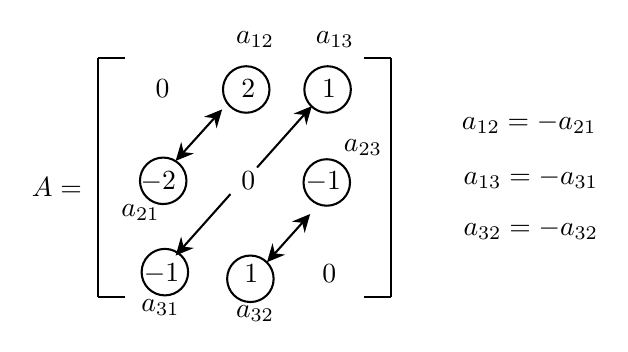
\begin{tikzpicture}[x=0.75pt,y=0.75pt,yscale=-0.8,xscale=0.8]
%uncomment if require: \path (0,300); %set diagram left start at 0, and has height of 300

%Straight Lines [id:da4447046460953976] 
\draw    (217.89,80) -- (217.89,224) ;
%Straight Lines [id:da7752964595152956] 
\draw    (217.89,80) -- (234,80) ;
%Straight Lines [id:da7155601980908994] 
\draw    (217.89,224) -- (234,224) ;

%Straight Lines [id:da7468025243759369] 
\draw    (394,224) -- (394,80) ;
%Straight Lines [id:da9506678455834403] 
\draw    (394,224) -- (377.89,224) ;
%Straight Lines [id:da11439279523706714] 
\draw    (394,80) -- (377.89,80) ;

%Straight Lines [id:da8629837273526277] 
\draw    (266.51,139.77) -- (290.49,113.23) ;
\draw [shift={(292.5,111)}, rotate = 492.09] [fill={rgb, 255:red, 0; green, 0; blue, 0 }  ][line width=0.08]  [draw opacity=0] (10.72,-5.15) -- (0,0) -- (10.72,5.15) -- (7.12,0) -- cycle    ;
\draw [shift={(264.5,142)}, rotate = 312.09] [fill={rgb, 255:red, 0; green, 0; blue, 0 }  ][line width=0.08]  [draw opacity=0] (10.72,-5.15) -- (0,0) -- (10.72,5.15) -- (7.12,0) -- cycle    ;
%Straight Lines [id:da582084814391653] 
\draw    (321.5,200.77) -- (343.5,176.23) ;
\draw [shift={(345.5,174)}, rotate = 491.88] [fill={rgb, 255:red, 0; green, 0; blue, 0 }  ][line width=0.08]  [draw opacity=0] (10.72,-5.15) -- (0,0) -- (10.72,5.15) -- (7.12,0) -- cycle    ;
\draw [shift={(319.5,203)}, rotate = 311.88] [fill={rgb, 255:red, 0; green, 0; blue, 0 }  ][line width=0.08]  [draw opacity=0] (10.72,-5.15) -- (0,0) -- (10.72,5.15) -- (7.12,0) -- cycle    ;
%Shape: Circle [id:dp8923484895491729] 
\draw   (293,99) .. controls (293,91.27) and (299.27,85) .. (307,85) .. controls (314.73,85) and (321,91.27) .. (321,99) .. controls (321,106.73) and (314.73,113) .. (307,113) .. controls (299.27,113) and (293,106.73) .. (293,99) -- cycle ;
%Shape: Circle [id:dp26541354623882585] 
\draw   (243,154) .. controls (243,146.27) and (249.27,140) .. (257,140) .. controls (264.73,140) and (271,146.27) .. (271,154) .. controls (271,161.73) and (264.73,168) .. (257,168) .. controls (249.27,168) and (243,161.73) .. (243,154) -- cycle ;
%Shape: Circle [id:dp3092729936725449] 
\draw   (342,99) .. controls (342,91.27) and (348.27,85) .. (356,85) .. controls (363.73,85) and (370,91.27) .. (370,99) .. controls (370,106.73) and (363.73,113) .. (356,113) .. controls (348.27,113) and (342,106.73) .. (342,99) -- cycle ;
%Shape: Circle [id:dp8496309320322011] 
\draw   (244,209) .. controls (244,201.27) and (250.27,195) .. (258,195) .. controls (265.73,195) and (272,201.27) .. (272,209) .. controls (272,216.73) and (265.73,223) .. (258,223) .. controls (250.27,223) and (244,216.73) .. (244,209) -- cycle ;
%Shape: Circle [id:dp2717937022569339] 
\draw   (341.5,155) .. controls (341.5,147.27) and (347.77,141) .. (355.5,141) .. controls (363.23,141) and (369.5,147.27) .. (369.5,155) .. controls (369.5,162.73) and (363.23,169) .. (355.5,169) .. controls (347.77,169) and (341.5,162.73) .. (341.5,155) -- cycle ;
%Shape: Circle [id:dp2552950220676966] 
\draw   (295.5,213) .. controls (295.5,205.27) and (301.77,199) .. (309.5,199) .. controls (317.23,199) and (323.5,205.27) .. (323.5,213) .. controls (323.5,220.73) and (317.23,227) .. (309.5,227) .. controls (301.77,227) and (295.5,220.73) .. (295.5,213) -- cycle ;
%Straight Lines [id:da8819386833529252] 
\draw    (297.5,162) -- (266.5,196.76) ;
\draw [shift={(264.5,199)}, rotate = 311.73] [fill={rgb, 255:red, 0; green, 0; blue, 0 }  ][line width=0.08]  [draw opacity=0] (10.72,-5.15) -- (0,0) -- (10.72,5.15) -- (7.12,0) -- cycle    ;
%Straight Lines [id:da8444500531478023] 
\draw    (344.5,111.24) -- (313.5,146) ;
\draw [shift={(346.5,109)}, rotate = 131.73] [fill={rgb, 255:red, 0; green, 0; blue, 0 }  ][line width=0.08]  [draw opacity=0] (10.72,-5.15) -- (0,0) -- (10.72,5.15) -- (7.12,0) -- cycle    ;

% Text Node
\draw (250.54,90.95) node [anchor=north west][inner sep=0.75pt]    {$0$};
% Text Node
\draw (302.2,90.95) node [anchor=north west][inner sep=0.75pt]    {$2$};
% Text Node
\draw (350.86,90.95) node [anchor=north west][inner sep=0.75pt]    {$1$};
% Text Node
\draw (241.54,146.4) node [anchor=north west][inner sep=0.75pt]    {$-2$};
% Text Node
\draw (302.2,146.4) node [anchor=north west][inner sep=0.75pt]    {$0$};
% Text Node
\draw (340.86,146.4) node [anchor=north west][inner sep=0.75pt]    {$-1$};
% Text Node
\draw (243.54,201.85) node [anchor=north west][inner sep=0.75pt]    {$-1$};
% Text Node
\draw (304,202.4) node [anchor=north west][inner sep=0.75pt]    {$1$};
% Text Node
\draw (351,202.4) node [anchor=north west][inner sep=0.75pt]    {$0$};
% Text Node
\draw (176,150.4) node [anchor=north west][inner sep=0.75pt]    {$A=$};
% Text Node
\draw (299,62.4) node [anchor=north west][inner sep=0.75pt]    {$a_{12}$};
% Text Node
\draw (230,166.4) node [anchor=north west][inner sep=0.75pt]    {$a_{21}$};
% Text Node
\draw (347,62.4) node [anchor=north west][inner sep=0.75pt]    {$a_{13}$};
% Text Node
\draw (242,223.4) node [anchor=north west][inner sep=0.75pt]    {$a_{31}$};
% Text Node
\draw (299,227.4) node [anchor=north west][inner sep=0.75pt]    {$a_{32}$};
% Text Node
\draw (364,127.4) node [anchor=north west][inner sep=0.75pt]    {$a_{23}$};
% Text Node
\draw (435,111.4) node [anchor=north west][inner sep=0.75pt]    {$a_{12} =-a_{21}$};
% Text Node
\draw (436,144.4) node [anchor=north west][inner sep=0.75pt]    {$a_{13} =-a_{31}$};
% Text Node
\draw (436,175.4) node [anchor=north west][inner sep=0.75pt]    {$a_{32} =-a_{32}$};


\end{tikzpicture}
		\caption{বিপ্রতিসম ম্যাট্রিক্স}
		\label{mat-fig-4}
	\end{figure}
	\begin{tcolorbox}
		\textbf{Note:} বিপ্রতিসম ম্যাট্রিক্স এর মুখ্য কর্ণের ভুক্তিগুলো শূন্য হয়।
	\end{tcolorbox}

	\item \textbf{হারমিশিয়ান ম্যাট্রিক্স (Hermitian Matrix):} কোনো ম্যাট্রিক্স $A=[a_{ij}]$ কে Hermitian Matrix বলা হবে যদি $a_{ij}=\overline{a_{ji}}$ হয় যেখানে $\overline{a_{ij}}$ দ্বারা $(i,j)$-তম ভুক্তির অনুবন্ধী জটিল সংখ্যা বুঝায়।\\ Example: $A=\left[\begin{array}{ccc}
		2 & 2+i & 4 \\
		2-i & 3 & i \\
		4 & -i & 1
		\end{array}\right]
		$।
	\begin{tcolorbox}
		\textbf{Note:}\\
		যেকোনো জটিল সংখ্যাকে $x=a+ib$ আকারে লেখা যায়।\\যেখানে, $a=$বাস্তব অংশ ও $b=$জটিল অংশ।\\ $x$ এর অনুবন্ধী জটিল সংখ্যা হবে $\bar{x}=a-ib$। \\অর্থাৎ জটিল অংশের চিহ্ন উল্টিয়ে দিলেই অনুবন্ধী পাওয়া যায়।\\ Example: 
		\begin{itemize}
			\item[$(i)$] $x=2+i$ হলে $\bar{x}=2-i$
			\item[$(ii)$] $x=2-3i$ হলে $\bar{x}=2+3i$
			\item[$(iii)$] $x=2$ হলে $\bar{x}=2$ (বাস্তব অংশের চিহ্ন পরিবর্তন হয় না)
		\end{itemize}
		(বিস্তারিত উচ্চতর গণিত ২য় পত্র জটিল সংখ্যা অধ্যায়) 
	\end{tcolorbox}	

	\item \textbf{স্কিউ-হারমিশিয়ান ম্যাট্রিক্স (Skew-Hermitian Matrix):} কোনো ম্যাট্রিক্স $A=[a_{ij}]$ কে Skew-Hermitian Matrix বলা হবে যদি $a_{ij}=-\overline{a_{ji}}$ হয় যেখানে $\overline{a_{ij}}$ দ্বারা $(i,j)$-তম ভুক্তির অনুবন্ধী জটিল সংখ্যা বুঝায়।\\ Example: 
	$A=\left[\begin{array}{ccc}
	i & 2+i & 3-4i \\
	-2+i & 0 & 4+5i \\
	-3-4i & -4+5i & 3i
	\end{array}\right]
	$।
	\\
	\item \textbf{উপ-ম্যাট্রিক্স (Sub-matrix):} কোনো ম্যাট্রিক্স এর যেকোনো সংখ্যক সারি ও কলাম এর ভুক্তি বাদ দিয়ে গঠিত ম্যাট্রিক্সকে মূল ম্যাট্রিক্স এর উপ-ম্যাট্রিক্স বলে।\\ Example: 
	$A=\left[\begin{array}{ccc}
	1 & 2 & 3 \\
	4 & 5 & 6 \\
	7 & 8 & 9
	\end{array}\right]$ ম্যাট্রিক্স এর উপ-ম্যাট্রিক্স\\ 
	$\left[\begin{array}{cc}
	1 & 2 \\
	4 & 5 
	\end{array}\right], 
	\left[\begin{array}{cc}
	2 & 3 \\
	5 & 6 
	\end{array}\right], 
	\left[\begin{array}{cc}
	1 & 2 \\
	4 & 5 \\
	7 & 8 
	\end{array}\right], 
	\left[\begin{array}{ccc}
	1 & 2 & 3\\
	4 & 5 & 6
	\end{array}\right]$।
	\\
	\item \textbf{বর্গ ম্যাট্রিক্সের ঘাতের উপর ভিত্তি করে কিছু প্রকারভেদঃ}
	\begin{tcolorbox}
		কোনো ম্যাট্রিক্স $A$ এর ঘাত $k$ বলতে বুঝায় ম্যাট্রিক্সটিকে $k$ সংখ্যকবার গুণ করা।
		অর্থাৎ $A^k=A.A\dots k\text{ সংখ্যক}$
	\end{tcolorbox}
	\begin{itemize}
		\item[$(i)$] \textbf{পিরিওডিক ম্যাট্রিক্স (Periodic Matrix):}\\ $A^k=A$ হলে, $A$ একটি পিরিওডিক ম্যাট্রিক্স যার পিরিয়ড $k$।\\ $k=2$ একে সমঘাতি ম্যাট্রিক্স (Idempotent Matrix) বলা হয়।\\ Example: $A=\left[\begin{array}{cc}
		1 & 0 \\
		0 & 1
		\end{array}\right]$ কারণ \\
		$A^2=A.A=\left[\begin{array}{cc}
		1 & 0 \\
		0 & 1
		\end{array}\right]=A$ 
		
		\item[$(ii)$] \textbf{অভেদঘাতি ম্যাট্রিক্স (Involutory Matrix):}\\ $A^2=A.A=I$ হলে, $A$ একটি অভেদঘাতি ম্যাট্রিক্স। \\Example: $A=\left[\begin{array}{rr}
		2 & 3 \\
		-1 & -2
		\end{array}\right]$ কারণ \\
		$A^2=A.A=\left[\begin{array}{rr}
		1 & 0 \\
		0 & 1
		\end{array}\right]=I$
		
		\item[$(iii)$] \textbf{শূন্যঘাতি ম্যাট্রিক্স (Nilpotent Matrix):}\\ ক্ষুদ্রতম স্বাভাবিক সংখ্যা $k$ এর জন্য $A^k$ শূন্য ম্যাট্রিক্স হলে $A$ একটি শুন্নঘাতি ম্যাট্রিক্স। এই $k$ কে শুন্নঘাতির সূচক বা ধাত (index) বলে। \\ Example: $A=\left[\begin{array}{cc}
		1 & -1 \\
		1 & -1
		\end{array}\right]$ কারণ\\
		$A^2=A.A=\left[\begin{array}{cc}
		0 & 0 \\
		0 & 0
		\end{array}\right]$; \\ সুতরাং $A$ একটি শুন্নঘাতি ম্যাট্রিক্স যার সূচক 2।
	\end{itemize}  
\end{enumerate}
\section{ম্যাট্রিক্স এর সমতা (Equality of Matrices)}\label{section-3}
দুইটি ম্যাট্রিক্স $A$ ও $B$ সমান হবে যদি ও কেবল যদি,
\begin{enumerate}
	\item $A$ ও $B$ এর ক্রম (order) সমান হয়।
	\item $A$ ও $B$ এর অনুরুপ ভুক্তিগুলো সমান হয়।
\end{enumerate}
\begin{figure}[h]
	\centering
	

\tikzset{every picture/.style={line width=0.75pt}} %set default line width to 0.75pt        

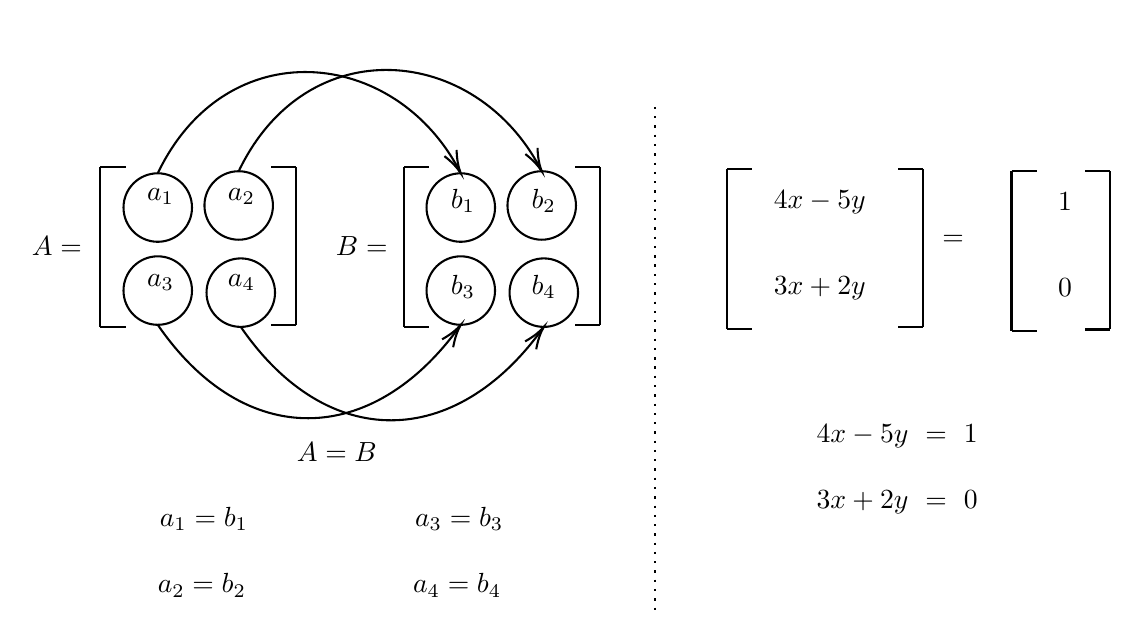
\begin{tikzpicture}[x=0.75pt,y=0.75pt,yscale=-1,xscale=1]
%uncomment if require: \path (0,300); %set diagram left start at 0, and has height of 300

%Straight Lines [id:da3998643853440913] 
\draw    (48.84,56) -- (48.84,133) ;
%Straight Lines [id:da4700304658953911] 
\draw    (48.84,56) -- (60.99,56) ;
%Straight Lines [id:da2189434943771349] 
\draw    (48.84,133) -- (60.99,133) ;

%Straight Lines [id:da042291976094193995] 
\draw    (143.19,132.25) -- (143.19,56) ;
%Straight Lines [id:da42742617171804187] 
\draw    (143.19,132.25) -- (131.04,132.25) ;
%Straight Lines [id:da6260416246879634] 
\draw    (143.19,56) -- (131.04,56) ;

%Straight Lines [id:da07775206432104698] 
\draw    (195.15,56) -- (195.15,133) ;
%Straight Lines [id:da9036238300369135] 
\draw    (195.15,56) -- (207.3,56) ;
%Straight Lines [id:da8945115880535983] 
\draw    (195.15,133) -- (207.3,133) ;

%Straight Lines [id:da1209242453210575] 
\draw    (289.5,132.25) -- (289.5,56) ;
%Straight Lines [id:da7693077584096126] 
\draw    (289.5,132.25) -- (277.35,132.25) ;
%Straight Lines [id:da02955184764396379] 
\draw    (289.5,56) -- (277.35,56) ;

%Shape: Circle [id:dp37093570591896685] 
\draw   (60,75.5) .. controls (60,66.39) and (67.39,59) .. (76.5,59) .. controls (85.61,59) and (93,66.39) .. (93,75.5) .. controls (93,84.61) and (85.61,92) .. (76.5,92) .. controls (67.39,92) and (60,84.61) .. (60,75.5) -- cycle ;
%Shape: Circle [id:dp43194785309147643] 
\draw   (99,74.5) .. controls (99,65.39) and (106.39,58) .. (115.5,58) .. controls (124.61,58) and (132,65.39) .. (132,74.5) .. controls (132,83.61) and (124.61,91) .. (115.5,91) .. controls (106.39,91) and (99,83.61) .. (99,74.5) -- cycle ;
%Shape: Circle [id:dp2549331909177619] 
\draw   (60,115.5) .. controls (60,106.39) and (67.39,99) .. (76.5,99) .. controls (85.61,99) and (93,106.39) .. (93,115.5) .. controls (93,124.61) and (85.61,132) .. (76.5,132) .. controls (67.39,132) and (60,124.61) .. (60,115.5) -- cycle ;
%Shape: Circle [id:dp5895564845905605] 
\draw   (100,116.5) .. controls (100,107.39) and (107.39,100) .. (116.5,100) .. controls (125.61,100) and (133,107.39) .. (133,116.5) .. controls (133,125.61) and (125.61,133) .. (116.5,133) .. controls (107.39,133) and (100,125.61) .. (100,116.5) -- cycle ;
%Shape: Circle [id:dp8078250776805984] 
\draw   (206,75.5) .. controls (206,66.39) and (213.39,59) .. (222.5,59) .. controls (231.61,59) and (239,66.39) .. (239,75.5) .. controls (239,84.61) and (231.61,92) .. (222.5,92) .. controls (213.39,92) and (206,84.61) .. (206,75.5) -- cycle ;
%Shape: Circle [id:dp7459823955845966] 
\draw   (245,74.5) .. controls (245,65.39) and (252.39,58) .. (261.5,58) .. controls (270.61,58) and (278,65.39) .. (278,74.5) .. controls (278,83.61) and (270.61,91) .. (261.5,91) .. controls (252.39,91) and (245,83.61) .. (245,74.5) -- cycle ;
%Shape: Circle [id:dp23256090829824472] 
\draw   (206,115.5) .. controls (206,106.39) and (213.39,99) .. (222.5,99) .. controls (231.61,99) and (239,106.39) .. (239,115.5) .. controls (239,124.61) and (231.61,132) .. (222.5,132) .. controls (213.39,132) and (206,124.61) .. (206,115.5) -- cycle ;
%Shape: Circle [id:dp6573871584758684] 
\draw   (246,116.5) .. controls (246,107.39) and (253.39,100) .. (262.5,100) .. controls (271.61,100) and (279,107.39) .. (279,116.5) .. controls (279,125.61) and (271.61,133) .. (262.5,133) .. controls (253.39,133) and (246,125.61) .. (246,116.5) -- cycle ;
%Curve Lines [id:da37234528213783946] 
\draw    (76.5,59) .. controls (109.34,-9.66) and (190.68,-2.08) .. (222.03,58.09) ;
\draw [shift={(222.5,59)}, rotate = 243.06] [color={rgb, 255:red, 0; green, 0; blue, 0 }  ][line width=0.75]    (10.93,-3.29) .. controls (6.95,-1.4) and (3.31,-0.3) .. (0,0) .. controls (3.31,0.3) and (6.95,1.4) .. (10.93,3.29)   ;
%Curve Lines [id:da901757426232622] 
\draw    (115.5,58) .. controls (148.34,-10.66) and (229.68,-3.08) .. (261.03,57.09) ;
\draw [shift={(261.5,58)}, rotate = 243.06] [color={rgb, 255:red, 0; green, 0; blue, 0 }  ][line width=0.75]    (10.93,-3.29) .. controls (6.95,-1.4) and (3.31,-0.3) .. (0,0) .. controls (3.31,0.3) and (6.95,1.4) .. (10.93,3.29)   ;
%Curve Lines [id:da09069426562891869] 
\draw    (76.5,132) .. controls (118.29,192.7) and (179.88,191.02) .. (221.87,132.88) ;
\draw [shift={(222.5,132)}, rotate = 485.45] [color={rgb, 255:red, 0; green, 0; blue, 0 }  ][line width=0.75]    (10.93,-3.29) .. controls (6.95,-1.4) and (3.31,-0.3) .. (0,0) .. controls (3.31,0.3) and (6.95,1.4) .. (10.93,3.29)   ;
%Curve Lines [id:da11878592161920998] 
\draw    (116.5,133) .. controls (158.29,193.7) and (219.88,192.02) .. (261.87,133.88) ;
\draw [shift={(262.5,133)}, rotate = 485.45] [color={rgb, 255:red, 0; green, 0; blue, 0 }  ][line width=0.75]    (10.93,-3.29) .. controls (6.95,-1.4) and (3.31,-0.3) .. (0,0) .. controls (3.31,0.3) and (6.95,1.4) .. (10.93,3.29)   ;
%Straight Lines [id:da31577321762510957] 
\draw    (350.84,57) -- (350.84,134) ;
%Straight Lines [id:da3136752541738428] 
\draw    (350.84,57) -- (362.99,57) ;
%Straight Lines [id:da10874809105993966] 
\draw    (350.84,134) -- (362.99,134) ;

%Straight Lines [id:da34615996972176166] 
\draw    (445.19,133.25) -- (445.19,57) ;
%Straight Lines [id:da09800818949598655] 
\draw    (445.19,133.25) -- (433.04,133.25) ;
%Straight Lines [id:da4567036877275019] 
\draw    (445.19,57) -- (433.04,57) ;

%Straight Lines [id:da4103484235620709] 
\draw    (487.84,58) -- (487.84,135) ;
%Straight Lines [id:da741377470998682] 
\draw    (487.84,58) -- (499.99,58) ;
%Straight Lines [id:da2558630207898225] 
\draw    (487.84,135) -- (499.99,135) ;

%Straight Lines [id:da8921390067578867] 
\draw    (535.19,134.25) -- (535.19,58) ;
%Straight Lines [id:da31495302630677346] 
\draw    (535.19,134.25) -- (523.04,134.25) ;
%Straight Lines [id:da837173507815582] 
\draw    (535.19,58) -- (523.04,58) ;

%Straight Lines [id:da5279355183178787] 
\draw  [dash pattern={on 0.84pt off 2.51pt}]  (316,27) -- (316,270) ;

% Text Node
\draw (69.86,65.01) node [anchor=north west][inner sep=0.75pt]    {$a_{1}$};
% Text Node
\draw (108.82,65.01) node [anchor=north west][inner sep=0.75pt]    {$a_{2}$};
% Text Node
\draw (69.86,106.46) node [anchor=north west][inner sep=0.75pt]    {$a_{3}$};
% Text Node
\draw (108.82,106.46) node [anchor=north west][inner sep=0.75pt]    {$a_{4}$};
% Text Node
\draw (14.33,88.02) node [anchor=north west][inner sep=0.75pt]    {$A=$};
% Text Node
\draw (216.17,65.01) node [anchor=north west][inner sep=0.75pt]    {$b_{1}$};
% Text Node
\draw (255.13,65.01) node [anchor=north west][inner sep=0.75pt]    {$b_{2}$};
% Text Node
\draw (216.17,106.46) node [anchor=north west][inner sep=0.75pt]    {$b_{3}$};
% Text Node
\draw (255.13,106.46) node [anchor=north west][inner sep=0.75pt]    {$b_{4}$};
% Text Node
\draw (160.88,88.02) node [anchor=north west][inner sep=0.75pt]    {$B=$};
% Text Node
\draw (142,187.4) node [anchor=north west][inner sep=0.75pt]    {$A=B$};
% Text Node
\draw (76,218.4) node [anchor=north west][inner sep=0.75pt]    {$a_{1} =b_{1}$};
% Text Node
\draw (75,250.4) node [anchor=north west][inner sep=0.75pt]    {$a_{2} =b_{2}$};
% Text Node
\draw (199,218.4) node [anchor=north west][inner sep=0.75pt]    {$a_{3} =b_{3}$};
% Text Node
\draw (198,250.4) node [anchor=north west][inner sep=0.75pt]    {$a_{4} =b_{4}$};
% Text Node
\draw (371.86,66.01) node [anchor=north west][inner sep=0.75pt]    {$4x-5y$};
% Text Node
\draw (371.86,107.46) node [anchor=north west][inner sep=0.75pt]    {$3x+2y$};
% Text Node
\draw (508.86,67.01) node [anchor=north west][inner sep=0.75pt]    {$1$};
% Text Node
\draw (508.86,108.46) node [anchor=north west][inner sep=0.75pt]    {$0$};
% Text Node
\draw (453,87.4) node [anchor=north west][inner sep=0.75pt]    {$=$};
% Text Node
\draw (388,178.4) node [anchor=north west][inner sep=0.75pt]    {$\therefore \ 4x-5y\ =\ 1$};
% Text Node
\draw (388,210.4) node [anchor=north west][inner sep=0.75pt]    {$\therefore \ 3x+2y\ =\ 0$};


\end{tikzpicture}
	\caption{ম্যাট্রিক্স এর সমতা}
	\label{mat-eq}
\end{figure}


\section{ম্যাট্রিক্স এর যোগ-বিয়োগ \\(Addition \& Subtraction of Matrices)}
যদি দুইটি একই ক্রমের ম্যাট্রিক্স 
$\color{red} A=
\left[\begin{array}{ccc}
a_1 & a_2 & a_3\\
a_4 & a_5 & a_6\\
a_7 & a_8 & a_9
\end{array}\right]$ ও $\color{blue}B=
\left[\begin{array}{ccc}
b_1 & b_2 & b_3\\
b_4 & b_5 & b_6\\
b_7 & b_8 & b_9
\end{array}\right]$ এর জন্য $\textcolor{red}{A}\pm \textcolor{blue}{B}=
\def \ra#1b#2{\textcolor{red}{a_{#1}}\pm\textcolor{blue}{b_{#2}}}
\left[\begin{array}{ccc}
\ra1b1 & \ra2b2 & \ra3b3\\
\ra4b4 & \ra5b5 & \ra6b6\\
\ra7b7 & \ra8b8 & \ra9b9
\end{array}\right]$।\\ Example: $
A=\left[\begin{array}{rr}
2 & -1 \\
3 & 6 
\end{array}\right]
$ ও $B=\left[\begin{array}{rr}
6 & 0 \\
5 & 3
\end{array}\right]$ হলে, $$\therefore A+B=\left[\begin{array}{rr}
2 & -1 \\
3 & 6 
\end{array}\right]+\left[\begin{array}{rr}
6 & 0 \\
5 & 3
\end{array}\right]=\left[\begin{array}{rr}
2+6 & -1+0 \\
3+5 & 6+3
\end{array}\right]=\left[\begin{array}{rr}
8 & -1\\
8 & 9
\end{array}\right]$$ 
$$\therefore A-B=\left[\begin{array}{rr}
2 & -1\\
3 & 6
\end{array}\right]-\left[\begin{array}{rr}
6 & 0\\
5 & 3
\end{array}\right]=\left[\begin{array}{rr}
2-6 & -1-0 \\
3-5 & 6-3 
\end{array}\right]=\left[\begin{array}{rr}
-4 & -1\\
-2 & 3
\end{array}\right]$$
\newpage
\section{ম্যাট্রিক্স এর গুণন (Multplication of Matrices)}
\subsection{ম্যাট্রিক্সের স্কেলার গুণিতক (Scalar Multiple of a Matrix)}\label{section-5-1}
কোনো ম্যাট্রিক্স $A$ কে কোনো একটি ধ্রুব সংখ্যা $k$ দ্বারা গুন করলে $kA$ ম্যাট্রিক্স এর প্রতিটি ভুক্তি $k$ দ্বারা গুন করতে হবে।\\ Example: 
$A=\left[\begin{array}{ccc}
a_{11} & a_{12} & a_{13} \\
a_{21} & a_{22} & a_{23} \\
a_{31} & a_{32} & a_{33}
\end{array}\right]$ হলে 
$\therefore kA=\left[\begin{array}{ccc}
ka_{11} & ka_{12} & ka_{13} \\
ka_{21} & ka_{22} & ka_{23} \\
ka_{31} & ka_{32} & ka_{33}
\end{array}\right]$।
\subsection{দুইটি ম্যাট্রিক্স এর গুণন (Multiplication of Two Matrices)}
\begin{tcolorbox}
	দুইটি ম্যাট্রিক্স $A$ ও $B$ গুণের শর্তঃ
	\begin{itemize}
		\item[$\diamond$] \textbf{$A$ এর কলাম সংখ্যা ও $B$ এর সারি সংখ্যা সমান হতে হবে।}
	\end{itemize}
	যদি $A$ এর ক্রম $m\times n$ এবং $B$ এর ক্রম $n\times l$ হয় তবে $AB$ সংজ্ঞায়িত কিন্তু $BA$ সংজ্ঞায়িত নয় কারণ $l\neq m$।
\end{tcolorbox}
\subsubsection{ম্যাট্রিক্স গুণের নিয়ম}
\begin{figure}
	\centering
	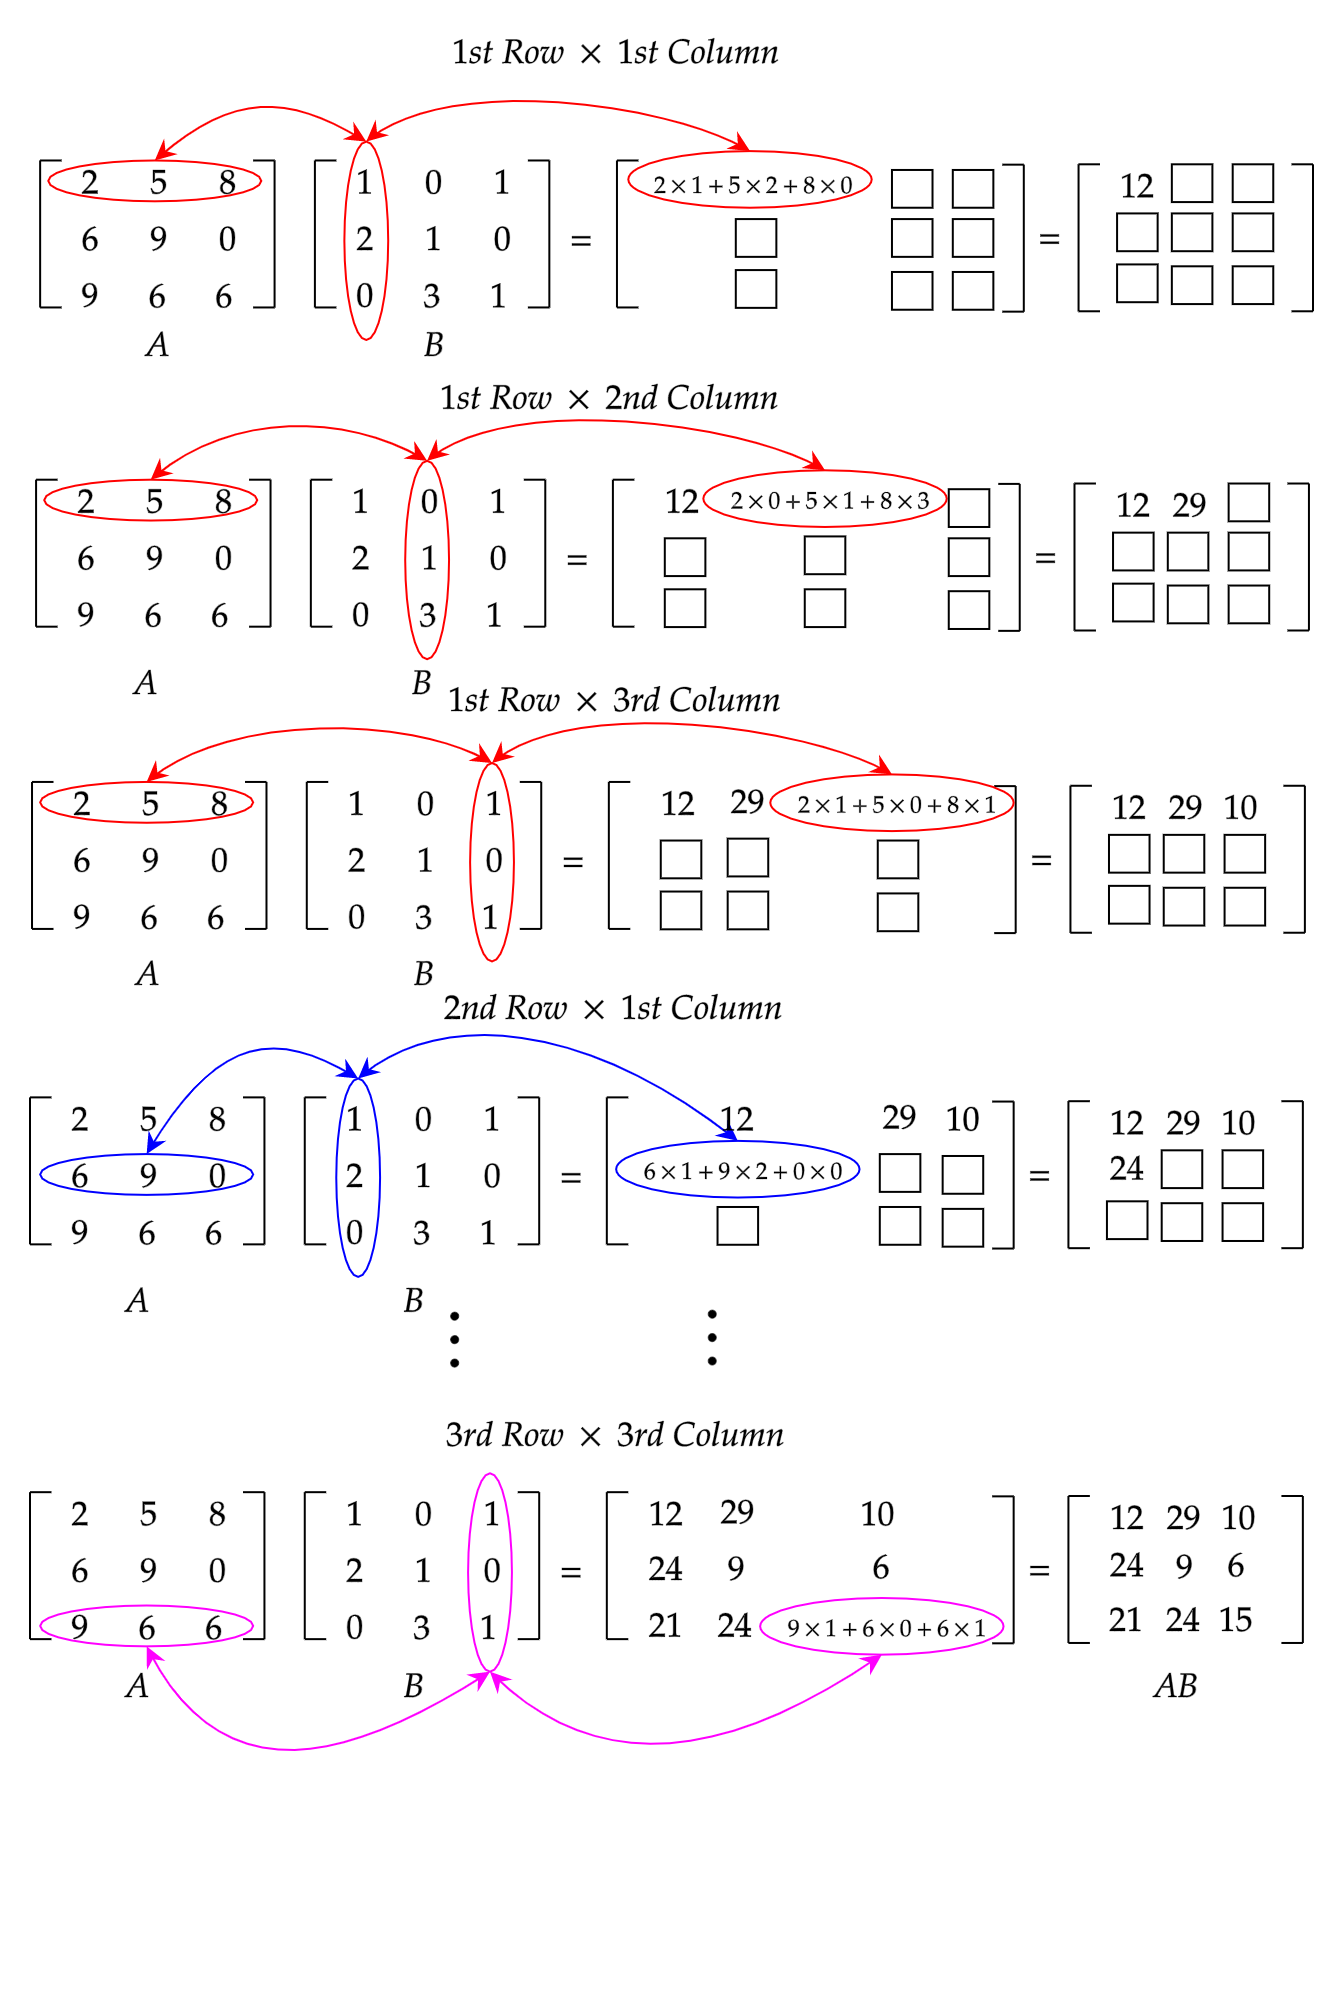
\includegraphics[scale=0.31]{images/matrix-mul.png}
	\caption{ম্যাট্রিক্স এর গুণন}
	\label{fig:matrix_mul}
\end{figure}
\begin{enumerate}
	\item $A$ ম্যাট্রিক্সের প্রথম সারির প্রতিটি ভুক্তি $B$ ম্যাট্রিক্সের প্রথম কলাম এর অনুরূপ ভুক্তির সাথে গুণ করতে হবে। এই গুণফলগুলির বীজগাণিতিক সমষ্টি হবে $AB$ ম্যাট্রিক্স এর প্রথম সারির প্রথম ভুক্তি। অনুরুপভাবে $A$ ম্যাট্রিক্সের ১ম সারির ভুক্তিগুলোকে যথাক্রমে $B$ ম্যাট্রিক্সের ২য় কলামের অনুরূপ ভুক্তিগুলোর সাথে গুণ করে যোগ করলে $AB$ ম্যাট্রিক্স এর ১ম সারির ২য় ভুক্তিটি পাওয়া যাবে। এভাবে অগ্রসর হয়ে $AB$ ম্যাট্রিক্সের ১ম সারির সবগুল ভুক্তি বের করতে হবে। (চিত্র \ref{fig:matrix_mul})
	\item নিয়ম ১ এর প্রক্রিয়ায় $AB$ এর সবগুল সারি নির্ণয় করতে হবে।	
\end{enumerate}
\newpage
Example: 
$\color{red} A=\left[\begin{array}{rrr}
1 & 0 & -2 \\
3 & -2 & -1
\end{array}\right]$ এবং 
$\color{blue} B=\left[\begin{array}{rr}
-1 & 3 \\
4 & 0 \\
2 & 6
\end{array}\right]$ হলে $AB$ ও $BA$ নির্ণয় কর।\\
Solution: যেহেতু $A$ এর ক্রম $2\times 3$ এবং $B$ এর ক্রম $3\times 2$ তাই $AB$ এবং $BA$ উভয় সংজ্ঞায়িত। \\  
$\therefore AB=\color{red}\left[\begin{array}{rrr}
1 & 0 & -2 \\
3 & -2 & -1
\end{array}\right]\color{blue}\left[\begin{array}{rr}
-1 & 3 \\
4 & 0 \\
2 & 6
\end{array}\right]$\\
$ \def \rb#1x#2{\textcolor{red}{#1}\times\textcolor{blue}{#2}}
=\left[\begin{array}{rrr}
\rb1x{-1} + \rb0x4 + \rb-2x2 & \rb1x3 + \rb0x0 + \rb-2x6 \\
\rb3x{-1} + \rb-2x4 + \rb-1x2 & \rb3x3 + \rb-2x0 + \rb-1x6 \\
\end{array}\right]$\\
$=\left[\begin{array}{rr}
-5 & -9 \\
-13 & 3
\end{array}\right]$\\
$\therefore BA=\color{blue}\left[\begin{array}{rr}
-1 & 3 \\
4 & 0 \\
2 & 6
\end{array}\right]\color{red}\left[\begin{array}{rrr}
1 & 0 & -2 \\
3 & -2 & -1
\end{array}\right]$\\
$ \def \br#1x#2{\textcolor{blue}{#1}\times\textcolor{red}{#2}}
=\left[\begin{array}{ccc}
\br-1x1+\br3x3 & \br-1x0+\br3x{-2} & \br-1x{-2}+\br3x{-1} \\
\br4x1+\br0x3 & \br4x0+\br0x{-2} & \br4x{-2}+\br0x{-1} \\
\br2x1+\br6x3 & \br2x0+\br6x{-2} & \br2x{-2}+\br6x{-1} 
\end{array}\right]$\\
$=\left[\begin{array}{rrr}
8 & -6 & -1 \\
4 & 0 & -8 \\
20 & -12 & -10
\end{array}\right]$
\begin{tcolorbox}
	\textbf{Note:} $A$ ও $B$ এর ক্রম যথাক্রমে $m\times n$ ও $n\times l$ হলে $AB$ এর ক্রম হবে $(m\times l)$
\end{tcolorbox}
\section{নির্ণায়ক এর সংজ্ঞা (Definition of Determinant)}
প্রত্যেক বর্গ ম্যাট্রিক্স সংশ্লিষ্ট একটি গুরুত্বপূর্ণ সংখারাশি রয়েছে যাকে ম্যাট্রিক্সটির নির্ণায়ক (Determinant) বলা হয়। কোনো ম্যাট্রিক্স 
$A=\left[\begin{array}{cc}
a_{1} & b_{1} \\
a_{2} & b_{2}
\end{array}\right]$ হলে এর নির্ণায়ককে $|A|$ বা $det(A)=\left|\begin{array}{cc}
a_{1} & b_{1} \\
a_{2} & b_{2}
\end{array}\right|$ দ্বারা প্রকাশ করা হয় যার মান $a_{1}b_{2}-a_{2}b_{1}$। অনুরুপভাবে 
$B=\left[\begin{array}{ccc}
a_{1} & b_{1} & c_{1} \\
a_{2} & b_{2} & c_{2} \\
a_{3} & b_{3} & c_{3}
\end{array}\right]$ ম্যাট্রিক্সটির নির্ণায়ক $|B|=det(B)=\left|\begin{array}{ccc}
a_{1} & b_{1} & c_{1} \\
a_{2} & b_{2} & c_{2} \\
a_{3} & b_{3} & c_{3}
\end{array}\right|$। 
\begin{tcolorbox}
	\begin{itemize}
		\item[$\bullet$] \textbf{নির্ণায়ক এর মুখ্যপদঃ} নির্ণায়ক এর মুখ্যকর্ণ বরাবর ভুক্তিগুলোর গুনফল।\\ Example: $|A|=\left|\begin{array}{ccc}
		\textcolor{red}{a_{1}} & b_{1} & c_{1} \\
		a_{2} & \textcolor{red}{b_{2}} & c_{2} \\
		a_{3} & b_{3} & \textcolor{red}{c_{3}}
		\end{array}\right|$ এর জন্য মুখ্যপদ  $\textcolor{red}{a_{1}b_{2}c_{3}}$।
		\item[$\bullet$] \textbf{নির্ণায়ক এর মাধ্যমিক পদঃ} নির্ণায়ক এর গৌণকর্ণ বরাবর ভুক্তিগুলোর গুনফল। Example: $|A|=\left|\begin{array}{ccc}
		a_{1} & b_{1} & \textcolor{red}{c_{1}} \\
		a_{2} & \textcolor{red}{b_{2}} & c_{2} \\
		\textcolor{red}{a_{3}} & b_{3} & c_{3}
		\end{array}\right|$ এর জন্য মাধ্যমিক পদ $\textcolor{red}{a_{3}b_{2}c_{1}}$। 
	\end{itemize}
\end{tcolorbox}
\subsection{নির্ণায়ক এর অনুরাশি ও সহগুণক (Minor \& Co-factor of determinant)}
\begin{itemize}
	\item[$\bullet$] \textbf{অনুরাশি (Minor):} কোনো নির্ণায়ক $|A|$ এর $(i,j)$-তম ভুক্তি $a_{ij}$ যে সারি ও যে কলামে অবস্থিত সে সারি $(i)$ ও সে কলাম $(j)$ ব্যাতীত অবশিষ্ট ভুক্তি দ্বারা গঠিত নির্ণায়ককে উক্ত ভুক্তির অনুরাশি (Minor) বলে।\\ 
		\begin{figure}[h]
		\centering
		

\tikzset{every picture/.style={line width=0.75pt}} %set default line width to 0.75pt        

\begin{tikzpicture}[x=0.75pt,y=0.75pt,yscale=-1,xscale=1]
%uncomment if require: \path (0,401); %set diagram left start at 0, and has height of 401

%Straight Lines [id:da31948622411951244] 
\draw    (90.89,14) -- (90.89,158) ;
%Straight Lines [id:da6593543662349199] 
\draw    (267,158) -- (267,14) ;
%Straight Lines [id:da45288949160346936] 
\draw    (90.89,183) -- (90.89,327) ;
%Straight Lines [id:da6668748376279647] 
\draw    (267,327) -- (267,183) ;
%Shape: Circle [id:dp22671069323852922] 
\draw   (108,34) .. controls (108,22.4) and (117.4,13) .. (129,13) .. controls (140.6,13) and (150,22.4) .. (150,34) .. controls (150,45.6) and (140.6,55) .. (129,55) .. controls (117.4,55) and (108,45.6) .. (108,34) -- cycle ;
%Straight Lines [id:da08065719677083094] 
\draw    (150,34) -- (257.5,34) ;
%Straight Lines [id:da9166990443765108] 
\draw    (129,55) -- (129,159) ;
%Straight Lines [id:da9318541142567531] 
\draw    (513.89,48) -- (513.89,123.26) ;
%Straight Lines [id:da344051477090638] 
\draw    (596.5,48.74) -- (596.5,124) ;
%Shape: Circle [id:dp3377944192427813] 
\draw   (159,257) .. controls (159,245.4) and (168.4,236) .. (180,236) .. controls (191.6,236) and (201,245.4) .. (201,257) .. controls (201,268.6) and (191.6,278) .. (180,278) .. controls (168.4,278) and (159,268.6) .. (159,257) -- cycle ;
%Straight Lines [id:da21410636837509145] 
\draw    (103.5,257) -- (159,257) ;
%Straight Lines [id:da5184450055549616] 
\draw    (201,257) -- (256.5,257) ;
%Straight Lines [id:da380019854201626] 
\draw    (180,236) -- (180,178) ;
%Straight Lines [id:da6912558298691118] 
\draw    (180,344) -- (180,278) ;
%Straight Lines [id:da06537782742261666] 
\draw    (517.89,216) -- (517.89,291.26) ;
%Straight Lines [id:da1736878921671534] 
\draw    (600.5,216.74) -- (600.5,292) ;

% Text Node
\draw (123.54,24.95) node [anchor=north west][inner sep=0.75pt]    {$2$};
% Text Node
\draw (175.2,24.95) node [anchor=north west][inner sep=0.75pt]    {$5$};
% Text Node
\draw (226.86,24.95) node [anchor=north west][inner sep=0.75pt]    {$8$};
% Text Node
\draw (123.54,80.4) node [anchor=north west][inner sep=0.75pt]    {$6$};
% Text Node
\draw (175.2,80.4) node [anchor=north west][inner sep=0.75pt]    {$9$};
% Text Node
\draw (226.86,80.4) node [anchor=north west][inner sep=0.75pt]    {$0$};
% Text Node
\draw (123.54,135.85) node [anchor=north west][inner sep=0.75pt]    {$9$};
% Text Node
\draw (174,136.4) node [anchor=north west][inner sep=0.75pt]    {$6$};
% Text Node
\draw (224,136.4) node [anchor=north west][inner sep=0.75pt]    {$6$};
% Text Node
\draw (50,76.4) node [anchor=north west][inner sep=0.75pt]    {$A=$};
% Text Node
\draw (123.54,193.95) node [anchor=north west][inner sep=0.75pt]    {$2$};
% Text Node
\draw (175.2,193.95) node [anchor=north west][inner sep=0.75pt]    {$5$};
% Text Node
\draw (226.86,193.95) node [anchor=north west][inner sep=0.75pt]    {$8$};
% Text Node
\draw (123.54,249.4) node [anchor=north west][inner sep=0.75pt]    {$6$};
% Text Node
\draw (175.2,249.4) node [anchor=north west][inner sep=0.75pt]    {$9$};
% Text Node
\draw (226.86,249.4) node [anchor=north west][inner sep=0.75pt]    {$0$};
% Text Node
\draw (123.54,304.85) node [anchor=north west][inner sep=0.75pt]    {$9$};
% Text Node
\draw (174,305.4) node [anchor=north west][inner sep=0.75pt]    {$6$};
% Text Node
\draw (224,305.4) node [anchor=north west][inner sep=0.75pt]    {$6$};
% Text Node
\draw (50,245.4) node [anchor=north west][inner sep=0.75pt]    {$A=$};
% Text Node
\draw (530.16,57.37) node [anchor=north west][inner sep=0.75pt]    {$9$};
% Text Node
\draw (570.81,57.37) node [anchor=north west][inner sep=0.75pt]    {$0$};
% Text Node
\draw (529.22,98.69) node [anchor=north west][inner sep=0.75pt]    {$6$};
% Text Node
\draw (568.56,98.69) node [anchor=north west][inner sep=0.75pt]    {$6$};
% Text Node
\draw (330,70) node [anchor=north west][inner sep=0.75pt] {$(1,1)$ তম  ভুক্তির  সহগুনক $=$};
% Text Node
\draw (534.16,225.37) node [anchor=north west][inner sep=0.75pt]    {$2$};
% Text Node
\draw (574.81,225.37) node [anchor=north west][inner sep=0.75pt]    {$8$};
% Text Node
\draw (533.22,266.69) node [anchor=north west][inner sep=0.75pt]    {$9$};
% Text Node
\draw (572.56,266.69) node [anchor=north west][inner sep=0.75pt]    {$6$};
% Text Node
\draw (330,240) node [anchor=north west][inner sep=0.75pt]  {$( 2,2)$ তম  ভুক্তির  সহগুনক $=$};

\end{tikzpicture}

		\caption{অনুরাশি (Minor)}
		\label{mat-fig-5}
	\end{figure}
	\newpage
	Example: \\ $\left|\begin{array}{cc}
	a_{11} & a_{12} \\
	a_{21} & a_{22}
	\end{array}\right|$ এর জন্য $a_{11}$ এর বা $(1,1)$-তম ভুক্তির অনুরাশি $|a_{22}|=a_{22}$।\\ 
	আবার
	$\left|\begin{array}{ccc}
	a_{11} & a_{12} & a_{13} \\
	a_{21} & a_{22} & a_{23} \\
	a_{31} & a_{32} & a_{33}
	\end{array}\right|$ এর জন্য $a_{11}$ এর বা \\$(1,1)$-তম ভুক্তির অনুরাশি $\left|\begin{array}{cc}
	a_{22} & a_{23} \\
	a_{32} & a_{33}
	\end{array}\right|=a_{22}a_{33}-a_{23}a_{32}$ 
	\begin{tcolorbox}
		\textbf{Note:} একটিমাত্র ভুক্তি সম্বলিত নির্ণায়ক এর মান ঐ ভুক্তির মানের সমান।
	\end{tcolorbox}
 	\item[$\bullet$] \textbf{সহগুণক (Co-factor):} কোনো নির্ণায়ক $|A|$ এর কোনো ভুক্তি $a_{ij}$ এর যথাযথ চিহ্নযুক্ত অনুরাশিকে ঐ ভুক্তির সহগুণক (Co-factor) বলে যাকে $A_{ij}$ দ্বারা প্রকাশ করা হয়। $(i,j)$-তম ভুক্তি $a_{ij}$ এর চিহ্ন হবে $(-1)^{i+j}$।\\
 	Example:\\ একটি $2\times 2$ নির্ণায়ক
 	$D\equiv\left|\begin{array}{cc}
 	d_{11} & d_{12} \\
 	d_{21} & d_{22}
 	\end{array}\right|$ এর ভুক্তিগুলোর সহগুণকগুলো যথাক্রমে \\
 	$D_{11}=(-1)^{1+1}\left|d_{22}\right|=d_{22}$ \\
 	$D_{12}=(-1)^{1+2}\left|d_{21}\right|=-d_{21}$ \\
 	$D_{21}=(-1)^{2+1}\left|d_{12}\right|=-d_{12}$ \\
 	$D_{22}=(-1)^{2+2}\left|d_{11}\right|=d_{11}$ \\
 	আবার একটি $3\times 3$ নির্ণায়ক 
 	$A\equiv\left|\begin{array}{ccc}
 	a_{11} & a_{12} & a_{13} \\
 	a_{21} & a_{22} & a_{23} \\
 	a_{31} & a_{32} & a_{33}
 	\end{array}\right|$ এর ভুক্তিগুলোর সহগুণকগুলো যথাক্রমে \\
 	$A_{11}=(-1)^{1+1}\left|\begin{array}{cc}
 	a_{22} & a_{23} \\
 	a_{32} & a_{33}
 	\end{array}\right|=\left|\begin{array}{cc}
 	a_{22} & a_{23} \\
 	a_{32} & a_{33}
 	\end{array}\right|=a_{22}a_{33}-a_{32}a_{23}$ \\
 	$A_{12}=(-1)^{1+2}\left|\begin{array}{cc}
 	a_{21} & a_{23} \\
 	a_{31} & a_{33}
 	\end{array}\right|=-\left|\begin{array}{cc}
 	a_{21} & a_{23} \\
 	a_{31} & a_{33}
 	\end{array}\right|=-(a_{21}a_{33}-a_{31}a_{23})$ \\
 	$A_{13}=(-1)^{1+3}\left|\begin{array}{cc}
 	a_{21} & a_{22} \\
 	a_{31} & a_{32}
 	\end{array}\right|=\left|\begin{array}{cc}
 	a_{21} & a_{22} \\
 	a_{31} & a_{32}
 	\end{array}\right|=a_{21}a_{32}-a_{31}a_{22}$ \\
 	$A_{21}=(-1)^{2+1}\left|\begin{array}{cc}
 	a_{12} & a_{13} \\
 	a_{32} & a_{33}
 	\end{array}\right|=-\left|\begin{array}{cc}
 	a_{12} & a_{13} \\
 	a_{32} & a_{33}
 	\end{array}\right|=-(a_{12}a_{33}-a_{32}a_{13})$ \\
 	$A_{22}=(-1)^{2+2}\left|\begin{array}{cc}
 	a_{11} & a_{13} \\
 	a_{31} & a_{33}
 	\end{array}\right|=\left|\begin{array}{cc}
 	a_{11} & a_{13} \\
 	a_{31} & a_{33}
 	\end{array}\right|=a_{11}a_{33}-a_{31}a_{13}$ \\
 	$A_{23}=(-1)^{2+3}\left|\begin{array}{cc}
 	a_{11} & a_{12} \\
 	a_{31} & a_{32}
 	\end{array}\right|=-\left|\begin{array}{cc}
 	a_{11} & a_{12} \\
 	a_{31} & a_{32}
 	\end{array}\right|=-(a_{11}a_{32}-a_{31}a_{12})$ \\
 	$A_{31}=(-1)^{3+1}\left|\begin{array}{cc}
 	a_{12} & a_{13} \\
 	a_{22} & a_{23}
 	\end{array}\right|=\left|\begin{array}{cc}
 	a_{12} & a_{13} \\
 	a_{22} & a_{23}
 	\end{array}\right|=a_{12}a_{23}-a_{22}a_{13}$ \\
 	$A_{32}=(-1)^{3+2}\left|\begin{array}{cc}
 	a_{11} & a_{13} \\
 	a_{21} & a_{23}
 	\end{array}\right|=-\left|\begin{array}{cc}
 	a_{11} & a_{13} \\
 	a_{21} & a_{23}
 	\end{array}\right|=-(a_{11}a_{23}-a_{21}a_{13})$ \\
 	$A_{33}=(-1)^{3+3}\left|\begin{array}{cc}
 	a_{11} & a_{12} \\
 	a_{21} & a_{22}
 	\end{array}\right|=\left|\begin{array}{cc}
 	a_{11} & a_{12} \\
 	a_{21} & a_{22}
 	\end{array}\right|=a_{11}a_{22}-a_{21}a_{12}$ \\
 	\begin{tcolorbox}
 		\textbf{Note:}
 		\begin{itemize}
 			\item[$\bullet$] $(i+j)$ জোড় হলে চিহ্ন $(+)$ এবং বিজোড় হলে চিহ্ন $(-)$ \\
 			\item[$\bullet$] $\left|\begin{array}{cc}
 				+ & - \\
 				- & +
 			\end{array}\right|_{2\times 2}, \left|\begin{array}{ccc}
 			+ & - & + \\
 			- & + & - \\
 			+ & - & +
 			\end{array}\right|_{3\times 3}, \left|\begin{array}{cccc}
 			+ & - & + & -\\
 			- & + & - & +\\
 			+ & - & + & - \\
 			- & + & - & +
 			\end{array}\right|_{4\times 4} $
 		\end{itemize}
 	\end{tcolorbox}
\end{itemize}

\section{নির্ণায়ক এর মান ও বিস্তৃতি \\(Value \& Expansion of Determinant)}\label{section-7}
কোনো নির্ণায়ক এর যেকোনো একটি সারি বা কলামের ভুক্তিসমূহ ও তাদের নিজ নিজ সহগুণকের গুণফলের সমষ্টিই নির্ণায়ক এর মান। \\
Example:\\
$
A \equiv \left|\begin{array}{cc}
a_{11} & a_{12} \\
a_{21} & a_{22}
\end{array}\right|=a_{11}A_{11}+a_{12}A_{12}=a_{11}a_{22}-a_{21}a_{12}
$
\\আবার,\\ 
$
	A\equiv\left|\begin{array}{ccc}
	a_{11} & a_{12} & a_{13} \\
	a_{21} & a_{22} & a_{23} \\
	a_{31} & a_{32} & a_{33}
	\end{array}\right|\\ \\
	=a_{11}A_{11}+a_{12}A_{12}+a_{13}A_{13}\\ \\
	=a_{11}\left|\begin{array}{cc}
	a_{22} & a_{23} \\
	a_{32} & a_{33}
	\end{array}\right|+a_{12}\times (-)\left|\begin{array}{cc}
	a_{21} & a_{23} \\
	a_{31} & a_{33}
	\end{array}\right|+a_{13}\left|\begin{array}{cc}
	a_{21} & a_{22} \\
	a_{31} & a_{32}
	\end{array}\right|
$
\subsection{সহগুণকের মাধ্যমে নির্ণায়ক এর বিস্তৃতি \\(Expansion of Determinant using Co-factor)}\label{exp-co-fact}
$D\equiv\left|\begin{array}{ccc}
a_1 & b_1 & c_1 \\
a_2 & b_2 & c_2 \\
a_3 & b_3 & c_3
\end{array}\right|$ নির্ণায়ক এর প্রথম সারির $a_1, b_1, c_1$ এর সহগুণক যথাক্রমে $A_1, B_1, C_1$। $\therefore D=a_1A_1+b_1B_1+c_1C_1$ (১ম সারি বরাবর বিস্তৃতি)\\
অনুরুপভাবে 
\begin{align*}
D &=a_2A_2+b_2B_2+c_2C_2 \hspace{5pt} & \text{ (২য় সারি বরাবর বিস্তৃতি)}\\
&=a_3A_3+b_3B_3+c_3C_3 \hspace{5pt} & \text{ (৩য় সারি বরাবর বিস্তৃতি)}\\
&=a_1A_1+a_2A_2+a_3A_3 \hspace{5pt} & \text{ (১ম কলাম বরাবর বিস্তৃতি)}\\
&=b_1B_1+b_2B_2+b_3B_3 \hspace{5pt} & \text{ (২য় কলাম বরাবর বিস্তৃতি)}\\
&=c_1C_1+c_2C_2+c_3C_3 \hspace{5pt} & \text{ (৩য় কলাম বরাবর বিস্তৃতি)}
\end{align*}
\subsection{সারাস চিত্রের মাধ্যমে নির্ণায়কের বিস্তৃতি \\(Expansion of Determinant Using Sarrus Diagram)}\label{sec-sarrus}
\begin{figure}[h]
	\centering
	\tikzset{every picture/.style={line width=0.75pt}} %set default line width to 0.75pt        

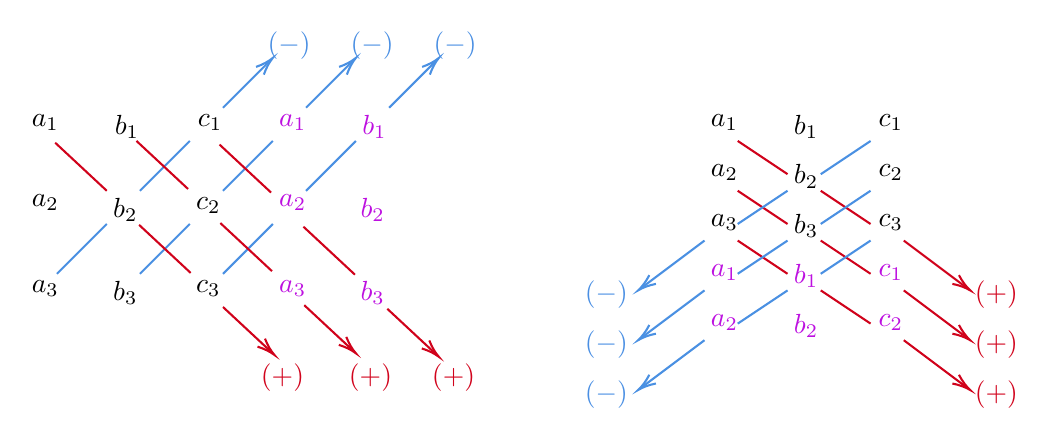
\begin{tikzpicture}[x=0.75pt,y=0.75pt,yscale=-0.8,xscale=0.8]
%uncomment if require: \path (0,300); %set diagram left start at 0, and has height of 300

%Straight Lines [id:da5748033318361949] 
\draw [color={rgb, 255:red, 74; green, 144; blue, 226 }  ,draw opacity=1 ]   (40,150) -- (70,120) ;
%Straight Lines [id:da8297838041597705] 
\draw [color={rgb, 255:red, 74; green, 144; blue, 226 }  ,draw opacity=1 ]   (90,100) -- (120,70) ;
%Straight Lines [id:da8299046802807408] 
\draw [color={rgb, 255:red, 74; green, 144; blue, 226 }  ,draw opacity=1 ]   (140,50) -- (168.59,21.41) ;
\draw [shift={(170,20)}, rotate = 495] [color={rgb, 255:red, 74; green, 144; blue, 226 }  ,draw opacity=1 ][line width=0.75]    (10.93,-3.29) .. controls (6.95,-1.4) and (3.31,-0.3) .. (0,0) .. controls (3.31,0.3) and (6.95,1.4) .. (10.93,3.29)   ;
%Straight Lines [id:da9479152542056342] 
\draw [color={rgb, 255:red, 74; green, 144; blue, 226 }  ,draw opacity=1 ]   (140,100) -- (170,70) ;
%Straight Lines [id:da7168172474748482] 
\draw [color={rgb, 255:red, 74; green, 144; blue, 226 }  ,draw opacity=1 ]   (190,50) -- (218.59,21.41) ;
\draw [shift={(220,20)}, rotate = 495] [color={rgb, 255:red, 74; green, 144; blue, 226 }  ,draw opacity=1 ][line width=0.75]    (10.93,-3.29) .. controls (6.95,-1.4) and (3.31,-0.3) .. (0,0) .. controls (3.31,0.3) and (6.95,1.4) .. (10.93,3.29)   ;
%Straight Lines [id:da1342542651652474] 
\draw [color={rgb, 255:red, 74; green, 144; blue, 226 }  ,draw opacity=1 ]   (90,150) -- (120,120) ;
%Straight Lines [id:da7867883166424012] 
\draw [color={rgb, 255:red, 74; green, 144; blue, 226 }  ,draw opacity=1 ]   (190,100) -- (220,70) ;
%Straight Lines [id:da6999100159782665] 
\draw [color={rgb, 255:red, 74; green, 144; blue, 226 }  ,draw opacity=1 ]   (240,50) -- (268.59,21.41) ;
\draw [shift={(270,20)}, rotate = 495] [color={rgb, 255:red, 74; green, 144; blue, 226 }  ,draw opacity=1 ][line width=0.75]    (10.93,-3.29) .. controls (6.95,-1.4) and (3.31,-0.3) .. (0,0) .. controls (3.31,0.3) and (6.95,1.4) .. (10.93,3.29)   ;
%Straight Lines [id:da0833246033058106] 
\draw [color={rgb, 255:red, 74; green, 144; blue, 226 }  ,draw opacity=1 ]   (140,150) -- (170,120) ;
%Straight Lines [id:da49398207340082045] 
\draw [color={rgb, 255:red, 208; green, 2; blue, 27 }  ,draw opacity=1 ]   (89.48,120.54) -- (120.52,149.46) ;
%Straight Lines [id:da8716745272222872] 
\draw [color={rgb, 255:red, 208; green, 2; blue, 27 }  ,draw opacity=1 ]   (140,170) -- (169.58,197.56) ;
\draw [shift={(171.04,198.92)}, rotate = 222.97] [color={rgb, 255:red, 208; green, 2; blue, 27 }  ,draw opacity=1 ][line width=0.75]    (10.93,-3.29) .. controls (6.95,-1.4) and (3.31,-0.3) .. (0,0) .. controls (3.31,0.3) and (6.95,1.4) .. (10.93,3.29)   ;
%Straight Lines [id:da8449078170090465] 
\draw [color={rgb, 255:red, 208; green, 2; blue, 27 }  ,draw opacity=1 ]   (38.96,71.08) -- (70,100) ;
%Straight Lines [id:da7329848671423627] 
\draw [color={rgb, 255:red, 208; green, 2; blue, 27 }  ,draw opacity=1 ]   (138.43,119.46) -- (169.48,148.38) ;
%Straight Lines [id:da1345141099064775] 
\draw [color={rgb, 255:red, 208; green, 2; blue, 27 }  ,draw opacity=1 ]   (188.96,168.92) -- (218.54,196.47) ;
\draw [shift={(220,197.84)}, rotate = 222.97] [color={rgb, 255:red, 208; green, 2; blue, 27 }  ,draw opacity=1 ][line width=0.75]    (10.93,-3.29) .. controls (6.95,-1.4) and (3.31,-0.3) .. (0,0) .. controls (3.31,0.3) and (6.95,1.4) .. (10.93,3.29)   ;
%Straight Lines [id:da7203260816975756] 
\draw [color={rgb, 255:red, 208; green, 2; blue, 27 }  ,draw opacity=1 ]   (87.91,70) -- (118.96,98.92) ;
%Straight Lines [id:da28669663908679843] 
\draw [color={rgb, 255:red, 208; green, 2; blue, 27 }  ,draw opacity=1 ]   (188.43,121.62) -- (219.48,150.54) ;
%Straight Lines [id:da18772907585823262] 
\draw [color={rgb, 255:red, 208; green, 2; blue, 27 }  ,draw opacity=1 ]   (238.96,171.08) -- (268.54,198.64) ;
\draw [shift={(270,200)}, rotate = 222.97] [color={rgb, 255:red, 208; green, 2; blue, 27 }  ,draw opacity=1 ][line width=0.75]    (10.93,-3.29) .. controls (6.95,-1.4) and (3.31,-0.3) .. (0,0) .. controls (3.31,0.3) and (6.95,1.4) .. (10.93,3.29)   ;
%Straight Lines [id:da7259932461629222] 
\draw [color={rgb, 255:red, 208; green, 2; blue, 27 }  ,draw opacity=1 ]   (137.91,72.16) -- (168.96,101.08) ;
%Straight Lines [id:da5836538440037218] 
\draw [color={rgb, 255:red, 208; green, 2; blue, 27 }  ,draw opacity=1 ]   (450,70) -- (469.73,83.15) -- (480,90) ;
%Straight Lines [id:da7338505693710413] 
\draw [color={rgb, 255:red, 208; green, 2; blue, 27 }  ,draw opacity=1 ]   (500,100) -- (530,120) ;
%Straight Lines [id:da05340083013981367] 
\draw [color={rgb, 255:red, 208; green, 2; blue, 27 }  ,draw opacity=1 ]   (550,130) -- (588.4,158.8) ;
\draw [shift={(590,160)}, rotate = 216.87] [color={rgb, 255:red, 208; green, 2; blue, 27 }  ,draw opacity=1 ][line width=0.75]    (10.93,-3.29) .. controls (6.95,-1.4) and (3.31,-0.3) .. (0,0) .. controls (3.31,0.3) and (6.95,1.4) .. (10.93,3.29)   ;
%Straight Lines [id:da44587233283485683] 
\draw [color={rgb, 255:red, 208; green, 2; blue, 27 }  ,draw opacity=1 ]   (450,100) -- (469.73,113.15) -- (480,120) ;
%Straight Lines [id:da9389636885235428] 
\draw [color={rgb, 255:red, 208; green, 2; blue, 27 }  ,draw opacity=1 ]   (500,130) -- (530,150) ;
%Straight Lines [id:da03468043106077001] 
\draw [color={rgb, 255:red, 208; green, 2; blue, 27 }  ,draw opacity=1 ]   (550,160) -- (588.4,188.8) ;
\draw [shift={(590,190)}, rotate = 216.87] [color={rgb, 255:red, 208; green, 2; blue, 27 }  ,draw opacity=1 ][line width=0.75]    (10.93,-3.29) .. controls (6.95,-1.4) and (3.31,-0.3) .. (0,0) .. controls (3.31,0.3) and (6.95,1.4) .. (10.93,3.29)   ;
%Straight Lines [id:da8452107596204068] 
\draw [color={rgb, 255:red, 208; green, 2; blue, 27 }  ,draw opacity=1 ]   (450,130) -- (469.73,143.15) -- (480,150) ;
%Straight Lines [id:da01662016421494683] 
\draw [color={rgb, 255:red, 208; green, 2; blue, 27 }  ,draw opacity=1 ]   (500,160) -- (530,180) ;
%Straight Lines [id:da8982258112751897] 
\draw [color={rgb, 255:red, 208; green, 2; blue, 27 }  ,draw opacity=1 ]   (550,190) -- (588.4,218.8) ;
\draw [shift={(590,220)}, rotate = 216.87] [color={rgb, 255:red, 208; green, 2; blue, 27 }  ,draw opacity=1 ][line width=0.75]    (10.93,-3.29) .. controls (6.95,-1.4) and (3.31,-0.3) .. (0,0) .. controls (3.31,0.3) and (6.95,1.4) .. (10.93,3.29)   ;
%Straight Lines [id:da42446180713663284] 
\draw [color={rgb, 255:red, 74; green, 144; blue, 226 }  ,draw opacity=1 ]   (530,70) -- (500,90) ;
%Straight Lines [id:da71403169389421] 
\draw [color={rgb, 255:red, 74; green, 144; blue, 226 }  ,draw opacity=1 ]   (480,100) -- (450,120) ;
%Straight Lines [id:da30413186098682066] 
\draw [color={rgb, 255:red, 74; green, 144; blue, 226 }  ,draw opacity=1 ]   (430,130) -- (391.6,158.8) ;
\draw [shift={(390,160)}, rotate = 323.13] [color={rgb, 255:red, 74; green, 144; blue, 226 }  ,draw opacity=1 ][line width=0.75]    (10.93,-3.29) .. controls (6.95,-1.4) and (3.31,-0.3) .. (0,0) .. controls (3.31,0.3) and (6.95,1.4) .. (10.93,3.29)   ;
%Straight Lines [id:da5245780389984886] 
\draw [color={rgb, 255:red, 74; green, 144; blue, 226 }  ,draw opacity=1 ]   (530,100) -- (500,120) ;
%Straight Lines [id:da5399987948821283] 
\draw [color={rgb, 255:red, 74; green, 144; blue, 226 }  ,draw opacity=1 ]   (480,130) -- (450,150) ;
%Straight Lines [id:da03398907406591012] 
\draw [color={rgb, 255:red, 74; green, 144; blue, 226 }  ,draw opacity=1 ]   (430,160) -- (391.6,188.8) ;
\draw [shift={(390,190)}, rotate = 323.13] [color={rgb, 255:red, 74; green, 144; blue, 226 }  ,draw opacity=1 ][line width=0.75]    (10.93,-3.29) .. controls (6.95,-1.4) and (3.31,-0.3) .. (0,0) .. controls (3.31,0.3) and (6.95,1.4) .. (10.93,3.29)   ;
%Straight Lines [id:da2601982135535541] 
\draw [color={rgb, 255:red, 74; green, 144; blue, 226 }  ,draw opacity=1 ]   (530,130) -- (500,150) ;
%Straight Lines [id:da1057578426618404] 
\draw [color={rgb, 255:red, 74; green, 144; blue, 226 }  ,draw opacity=1 ]   (480,160) -- (450,180) ;
%Straight Lines [id:da15043669894933265] 
\draw [color={rgb, 255:red, 74; green, 144; blue, 226 }  ,draw opacity=1 ]   (430,190) -- (391.6,218.8) ;
\draw [shift={(390,220)}, rotate = 323.13] [color={rgb, 255:red, 74; green, 144; blue, 226 }  ,draw opacity=1 ][line width=0.75]    (10.93,-3.29) .. controls (6.95,-1.4) and (3.31,-0.3) .. (0,0) .. controls (3.31,0.3) and (6.95,1.4) .. (10.93,3.29)   ;

% Text Node
\draw (23,52.4) node [anchor=north west][inner sep=0.75pt]    {$a_{1}$};
% Text Node
\draw (73,52.4) node [anchor=north west][inner sep=0.75pt]    {$b_{1}$};
% Text Node
\draw (23,100.4) node [anchor=north west][inner sep=0.75pt]    {$a_{2}$};
% Text Node
\draw (72,102.4) node [anchor=north west][inner sep=0.75pt]    {$b_{2}$};
% Text Node
\draw (23,152.4) node [anchor=north west][inner sep=0.75pt]    {$a_{3}$};
% Text Node
\draw (72,152.4) node [anchor=north west][inner sep=0.75pt]    {$b_{3}$};
% Text Node
\draw (123,52.4) node [anchor=north west][inner sep=0.75pt]    {$c_{1}$};
% Text Node
\draw (122,102.4) node [anchor=north west][inner sep=0.75pt]    {$c_{2}$};
% Text Node
\draw (122,152.4) node [anchor=north west][inner sep=0.75pt]    {$c_{3}$};
% Text Node
\draw (172,52.4) node [anchor=north west][inner sep=0.75pt]  [color={rgb, 255:red, 189; green, 16; blue, 224 }  ,opacity=1 ]  {$a_{1}$};
% Text Node
\draw (222,52.4) node [anchor=north west][inner sep=0.75pt]  [color={rgb, 255:red, 189; green, 16; blue, 224 }  ,opacity=1 ]  {$b_{1}$};
% Text Node
\draw (172,100.4) node [anchor=north west][inner sep=0.75pt]  [color={rgb, 255:red, 189; green, 16; blue, 224 }  ,opacity=1 ]  {$a_{2}$};
% Text Node
\draw (221,102.4) node [anchor=north west][inner sep=0.75pt]  [color={rgb, 255:red, 189; green, 16; blue, 224 }  ,opacity=1 ]  {$b_{2}$};
% Text Node
\draw (172,152.4) node [anchor=north west][inner sep=0.75pt]  [color={rgb, 255:red, 189; green, 16; blue, 224 }  ,opacity=1 ]  {$a_{3}$};
% Text Node
\draw (221,152.4) node [anchor=north west][inner sep=0.75pt]  [color={rgb, 255:red, 189; green, 16; blue, 224 }  ,opacity=1 ]  {$b_{3}$};
% Text Node
\draw (161,202.4) node [anchor=north west][inner sep=0.75pt]    {$\textcolor[rgb]{0.82,0.01,0.11}{( +)}$};
% Text Node
\draw (214,202.4) node [anchor=north west][inner sep=0.75pt]    {$\textcolor[rgb]{0.82,0.01,0.11}{(}\textcolor[rgb]{0.82,0.01,0.11}{+}\textcolor[rgb]{0.82,0.01,0.11}{)}$};
% Text Node
\draw (264,202.4) node [anchor=north west][inner sep=0.75pt]    {$\textcolor[rgb]{0.82,0.01,0.11}{(}\textcolor[rgb]{0.82,0.01,0.11}{+}\textcolor[rgb]{0.82,0.01,0.11}{)}$};
% Text Node
\draw (165,2.4) node [anchor=north west][inner sep=0.75pt]    {$\textcolor[rgb]{0.29,0.56,0.89}{( -)}$};
% Text Node
\draw (265,2.4) node [anchor=north west][inner sep=0.75pt]    {$\textcolor[rgb]{0.29,0.56,0.89}{(}\textcolor[rgb]{0.29,0.56,0.89}{-}\textcolor[rgb]{0.29,0.56,0.89}{)}$};
% Text Node
\draw (215,2.4) node [anchor=north west][inner sep=0.75pt]    {$\textcolor[rgb]{0.29,0.56,0.89}{(}\textcolor[rgb]{0.29,0.56,0.89}{-}\textcolor[rgb]{0.29,0.56,0.89}{)}$};
% Text Node
\draw (432,52.4) node [anchor=north west][inner sep=0.75pt]    {$a_{1}$};
% Text Node
\draw (482,52.4) node [anchor=north west][inner sep=0.75pt]    {$b_{1}$};
% Text Node
\draw (533,52.4) node [anchor=north west][inner sep=0.75pt]    {$c_{1}$};
% Text Node
\draw (432,82.4) node [anchor=north west][inner sep=0.75pt]    {$a_{2}$};
% Text Node
\draw (482,82.4) node [anchor=north west][inner sep=0.75pt]    {$b_{2}$};
% Text Node
\draw (533,82.4) node [anchor=north west][inner sep=0.75pt]    {$c_{2}$};
% Text Node
\draw (432,112.4) node [anchor=north west][inner sep=0.75pt]    {$a_{3}$};
% Text Node
\draw (482,112.4) node [anchor=north west][inner sep=0.75pt]    {$b_{3}$};
% Text Node
\draw (533,112.4) node [anchor=north west][inner sep=0.75pt]    {$c_{3}$};
% Text Node
\draw (432,142.4) node [anchor=north west][inner sep=0.75pt]  [color={rgb, 255:red, 189; green, 16; blue, 224 }  ,opacity=1 ]  {$a_{1}$};
% Text Node
\draw (482,142.4) node [anchor=north west][inner sep=0.75pt]  [color={rgb, 255:red, 189; green, 16; blue, 224 }  ,opacity=1 ]  {$b_{1}$};
% Text Node
\draw (533,142.4) node [anchor=north west][inner sep=0.75pt]  [color={rgb, 255:red, 189; green, 16; blue, 224 }  ,opacity=1 ]  {$c_{1}$};
% Text Node
\draw (432,172.4) node [anchor=north west][inner sep=0.75pt]  [color={rgb, 255:red, 189; green, 16; blue, 224 }  ,opacity=1 ]  {$a_{2}$};
% Text Node
\draw (482,172.4) node [anchor=north west][inner sep=0.75pt]  [color={rgb, 255:red, 189; green, 16; blue, 224 }  ,opacity=1 ]  {$b_{2}$};
% Text Node
\draw (533,172.4) node [anchor=north west][inner sep=0.75pt]  [color={rgb, 255:red, 189; green, 16; blue, 224 }  ,opacity=1 ]  {$c_{2}$};
% Text Node
\draw (591,212.4) node [anchor=north west][inner sep=0.75pt]    {$\textcolor[rgb]{0.82,0.01,0.11}{(}\textcolor[rgb]{0.82,0.01,0.11}{+}\textcolor[rgb]{0.82,0.01,0.11}{)}$};
% Text Node
\draw (591,182.4) node [anchor=north west][inner sep=0.75pt]    {$\textcolor[rgb]{0.82,0.01,0.11}{(}\textcolor[rgb]{0.82,0.01,0.11}{+}\textcolor[rgb]{0.82,0.01,0.11}{)}$};
% Text Node
\draw (591,152.4) node [anchor=north west][inner sep=0.75pt]    {$\textcolor[rgb]{0.82,0.01,0.11}{(}\textcolor[rgb]{0.82,0.01,0.11}{+}\textcolor[rgb]{0.82,0.01,0.11}{)}$};
% Text Node
\draw (356,152.4) node [anchor=north west][inner sep=0.75pt]    {$\textcolor[rgb]{0.29,0.56,0.89}{(}\textcolor[rgb]{0.29,0.56,0.89}{-}\textcolor[rgb]{0.29,0.56,0.89}{)}$};
% Text Node
\draw (356,182.4) node [anchor=north west][inner sep=0.75pt]    {$\textcolor[rgb]{0.29,0.56,0.89}{(}\textcolor[rgb]{0.29,0.56,0.89}{-}\textcolor[rgb]{0.29,0.56,0.89}{)}$};
% Text Node
\draw (356,212.4) node [anchor=north west][inner sep=0.75pt]    {$\textcolor[rgb]{0.29,0.56,0.89}{(}\textcolor[rgb]{0.29,0.56,0.89}{-}\textcolor[rgb]{0.29,0.56,0.89}{)}$};


\end{tikzpicture}
	\caption{$3\times 3$ নির্ণায়কের সারাস চিত্র}
	\label{fig:sarrus}
\end{figure}
কোনো ম্যাট্রিক্স 
$\left|\begin{array}{ccc}
a_1 & b_1 & c_1 \\
a_2 & b_2 & c_2 \\
a_3 & b_3 & c_3
\end{array}\right|$ এর মান $D$ দ্বারা সূচিত হলে সারাস চিত্র (চিত্র \ref{fig:sarrus}) অনুযায়ী লাল রেখা বরাবর গুণ করলে $(+)$ চিহ্নযুক্ত পদগুলো পাওয়া যায় এবং নীল রেখাগুলো বরাবর গুণ করলে $(-)$ চিহ্নযুক্ত পদগুলো পাওয়া যায়।\\
$D=\textcolor{red}{a_1b_2c_3+b_1c_2a_3+c_1a_2b_3}-(\textcolor{blue}{a_3b_2c_1+b_3c_2a_1+c_3a_2b_1})$

\section{নির্ণায়ক এর ধর্মাবলী (Properties of Determinant)}\label{section-8} 
\begin{enumerate}
	\item \textbf{নির্ণায়ক এর কোনো কলাম বা সারির প্রতিটি ভুক্তি শূন্য হলে নির্ণায়ক এর মান শূন্য হবে।}\label{prop-1}

	$\left|\begin{array}{ccc}
	0 & b_1 & c_1 \\
	0 & b_2 & c_2 \\
	0 & b_3 & c_3
	\end{array}\right|=0, 
	\left|\begin{array}{ccc}
	0 & 0 & 0 \\
	a_2 & b_2 & c_2 \\
	a_3 & b_3 & c_3
	\end{array}\right|=0$

	\item \textbf{নির্ণায়ক এর সারিকে কলাম এবং কলামকে সারিতে পরিবর্তন করলে নির্ণায়ক এর মান একই থাকে।}\label{prop-2}

	$\left|\begin{array}{ccc}
		a_1 & b_1 & c_1 \\
		a_2 & b_2 & c_2 \\
		a_3 & b_3 & c_3
	\end{array}\right|=\left|\begin{array}{ccc}
	a_1 & a_2 & a_3 \\
	b_1 & b_2 & b_3 \\
	c_1 & c_2 & c_3
	\end{array}\right|$
	

	\item \textbf{নির্ণায়কের দুইটি সারি অথবা কলাম পরস্পর স্থান বিনিময় করলে নির্ণায়ক এর চিহ্ন পরিবর্তিত হয় কিন্তু সাংখ্যিক মান একই থাকে।}\label{prop-3}

	$\left|\begin{array}{ccc}
	a_1 & b_1 & c_1 \\
	a_2 & b_2 & c_2 \\
	a_3 & b_3 & c_3
	\end{array}\right|=-\left|\begin{array}{ccc}
	a_2 & b_2 & c_2 \\
	a_1 & b_1 & c_1 \\
	a_3 & b_3 & c_3
	\end{array}\right|$ এবং $\left|\begin{array}{ccc}
	a_1 & b_1 & c_1 \\
	a_2 & b_2 & c_2 \\
	a_3 & b_3 & c_3
	\end{array}\right|=-\left|\begin{array}{ccc}
	b_1 & a_1 & c_1 \\
	b_2 & a_2 & c_2 \\
	b_3 & a_3 & c_3
	\end{array}\right|$
	\begin{tcolorbox}
		\begin{corollary}
			এই ধর্মের পর্যায়ক্রমিক প্রয়োগের দ্বারা একটি কলাম বা একটি সারিকে এক অবস্থান থেকে অন্য যেকোনো অবস্থানে নেয়া যায়। একবারে শুধুমাত্র দুইটি কলাম বা সারিতে এটি প্রয়োগ করা যাবে।
		\end{corollary}	
	\end{tcolorbox}

	\item \textbf{নির্ণায়কের দুইটি সারি বা দুইটি কলাম সমান হলে নির্ণায়ক এর মান শূন্য হবে।}\label{prop-4}
	
	$\left|\begin{array}{ccc}
		a_1 & a_1 & c_1 \\
		a_2 & a_2 & c_2 \\
		a_3 & a_3 & c_3
	\end{array}\right|=0, \left|\begin{array}{ccc}
	a_1 & b_1 & c_1 \\
	a_1 & b_1 & c_1 \\
	a_3 & b_3 & c_3
	\end{array}\right|=0$
	
	\item \textbf{নির্ণায়কের কোনো কলাম বা সারির ভুক্তিগুলো কোনো নির্দিষ্ট সংখ্যা দ্বারা করলে, নির্ণায়কের মানও ঐ সংখ্যা দ্বারা গুণ হয়।}\label{prop-5}

	$\left|\begin{array}{ccc}
	ma_1 & b_1 & c_1 \\
	ma_1 & b_1 & c_1 \\
	ma_3 & b_3 & c_3
	\end{array}\right|=m\left|\begin{array}{ccc}
	a_1 & b_1 & c_1 \\
	a_1 & b_1 & c_1 \\
	a_3 & b_3 & c_3
	\end{array}\right|$ \\  \\অনুরুপভাবে, $\left|\begin{array}{ccc}
	ma_1 & mb_1 & mc_1 \\
	a_1 & b_1 & c_1 \\
	a_3 & b_3 & c_3
	\end{array}\right|=m\left|\begin{array}{ccc}
	a_1 & b_1 & c_1 \\
	a_1 & b_1 & c_1 \\
	a_3 & b_3 & c_3
	\end{array}\right|$
	
	\item \textbf{নির্ণায়কের কোনো সারি বা কলাম এর ভুক্তিগুলোর সাথে অপর কোনো সারি বা কলাম এর সংশ্লিষ্ট সহগুণকগুলি দ্বারা যথাক্রমে গুণ করলে প্রাপ্ত গুণফলগুলোর বীজগাণিতিক সমষ্টি শূন্য হবে।}\label{prop-6}

	$D=\left|\begin{array}{ccc}
	a_1 & b_1 & c_1 \\
	a_1 & b_1 & c_1 \\
	a_3 & b_3 & c_3
	\end{array}\right|$ এর জন্য \\ \\
	$\begin{array}{cc}
	a_1A_2+b_1B_2+c_1C_2=0, & a_2A_3+b_2B_3+c_2C_3=0, \\
	a_3A_1+b_3B_1+c_3C_1=0, & a_1A_3+a_2A_1+a_3A_2=0, \\
	\cdots \quad \cdots,		& c_1C_3+c_2C_1+c_3C_2=0
	\end{array}$
	
	\item \textbf{নির্ণায়ক এর একটি সারি বা কলাম এর ভুক্তিগুলোর প্রত্যেকটি দুইটি ভুক্তির বীজগাণিতিক সমষ্টিরুপে গঠিত হলে, ঐ নির্ণায়কটিকে দুইটি নির্ণায়ক এর বীজগাণিতিক সমষ্টি আকারে প্রকাশ করা যায়।}\label{prop-7}

	$\left|\begin{array}{ccc}
	a_{1}\pm \alpha_{1} & b_{1} & c_{1} \\
	a_{2}\pm \alpha_{2} & b_{2} & c_{2} \\
	a_{3}\pm \alpha_{3} & b_{3} & c_{3}
	\end{array}\right|=\left|\begin{array}{ccc}
	a_{1} & b_{1} & c_{1} \\
	a_{2} & b_{2} & c_{2} \\
	a_{3} & b_{3} & c_{3}
	\end{array}\right| \pm \left|\begin{array}{ccc}
	\alpha_{1} & b_{1} & c_{1} \\
	\alpha_{2} & b_{2} & c_{2} \\
	\alpha_{3} & b_{3} & c_{3}
	\end{array}\right|$\\ \\
	অনুরুপভাবে, \\
	$\left|\begin{array}{ccc}
	a_{1}\pm \alpha_{1} & b_{1}\pm\alpha_{2} & c_{1}\pm\alpha_{3} \\
	a_{2} & b_{2} & c_{2} \\
	a_{3} & b_{3} & c_{3}
	\end{array}\right|=\left|\begin{array}{ccc}
	a_{1} & b_{1} & c_{1} \\
	a_{2} & b_{2} & c_{2} \\
	a_{3} & b_{3} & c_{3}
	\end{array}\right|\pm\left|\begin{array}{ccc}
	\alpha_{1} & \alpha_{2} & \alpha_{3} \\
	a_{2} & b_{2} & c_{2} \\
	a_{3} & b_{3} & c_{3}
	\end{array}\right|$
	
	\item \textbf{নির্ণায়কের একটি সারি বা কলামের প্রত্যেকটি ভুক্তিকে একটি নির্দিষ্ট সংখ্যা দ্বারা গুণ করে অপর কোনো সারি বা কলামের অনুরূপ ভুক্তিগুলোর সাথে যোগ বা বিয়োগ করলে নির্ণায়ক এর মান একই থাকে।}\label{prop-8}

	$\left|\begin{array}{ccc}
		a_{1} & b_{1} & c_{1} \\
		a_{2} & b_{2} & c_{2} \\
		a_{3} & b_{3} & c_{3}
	\end{array}\right|=\left|\begin{array}{ccc}
		a_{1} \pm m b_{1} & b_{1} & c_{1} \\
		a_{2} \pm m b_{2} & b_{2} & c_{2} \\
		a_{3} \pm m b_{3} & b_{3} & c_{3}
	\end{array}\right|$ $\pmb{\left[c'_1 = c_1 \pm mc_2\right]}$\\
	অনুরুপভাবে, 
	$\left|\begin{array}{ccc}
	a_{1} & b_{1} & c_{1} \\
	a_{2} & b_{2} & c_{2} \\
	a_{3} & b_{3} & c_{3}
	\end{array}\right|=\left|\begin{array}{ccc}
	a_{1} \pm m a_{2} & b_{1} \pm m b_{2} & c_{1}\pm m c_{2} \\
	a_{2}  & b_{2} & c_{2} \\
	a_{3}  & b_{3} & c_{3}
	\end{array}\right|$ $\pmb{\left[r'_1 = r_1 \pm mr_2\right]}$
\begin{tcolorbox}
 \textbf{Note:} নির্ণায়কের সারিগুলোকে $r_1,r_2,r_3,\cdots$ দ্বারা প্রকাশ করা হলে উপরুক্ত ধর্মগুলো প্রয়োগ করার পর সারিগুলোকে $r'_1,r'_2,r'_3,\cdots$ দ্বারা প্রকাশ করা হয়। কলাম এর ক্ষেত্রে $c'_1,c'_2,c'_3,\cdots$ দ্বারা প্রকাশ করা হয়।
\end{tcolorbox}
\end{enumerate}
\section{ব্যতিক্রমী, অব্যতিক্রমী ও অনুবন্ধী ম্যাট্রিক্স \\(Singular, Non-singular \& Adjoint Matrix)}
\begin{tcolorbox}[colback=green!5!white,colframe=green!75!black,title=\textbf{ব্যতিক্রমী ও অব্যতিক্রমী ম্যাট্রিক্স (Singular \& Non-singular Matrix)}]
	 \textbf{সংজ্ঞাঃ} যে সকল বর্গ ম্যাট্রিক্স এর নির্ণায়কের মান শূন্য তাদের ব্যাতিক্রমী (Singular) এবং যে সকল বর্গ ম্যাট্রিক্সের নির্ণায়কের মান অশূন্য তাদের অব্যতিক্রমী (Non-singular) ম্যাট্রিক্স বলে।
\end{tcolorbox}
মনেকরি, $A=[a_{ij}]_{m \times m}$ একটি বর্গ ম্যাট্রিক্স যার নির্ণায়ক কে $|A|=|a_{ij}|_{m \times m}$ দ্বারা প্রকাশ করা হয়।\\
যদি $|A|=0$ হয়, তবে $A$ ম্যাট্রিক্সটি ব্যতিক্রমী (Singular)। \\
যদি $|A|\neq 0$ হয়, তবে $A$ ম্যাট্রিক্সটি অব্যতিক্রমী (Non-singular)।\\
Example: \\ \\
$A=\left[\begin{array}{ccc}
1 & 2 & 3 \\
4 & 5 & 6 \\
7 & 8 & 9
\end{array}\right]$ ম্যাট্রিক্সটি নির্ণায়ক,\\ \\
$\therefore |A|=\left|\begin{array}{ccc}
1 & 2 & 3 \\
4 & 5 & 6 \\
7 & 8 & 9
\end{array}\right|=1(45-48)-2(36-42)+3(32-35)=-3+12-9=0$\\ \\
$\therefore A$ ম্যাট্রিক্সটি ব্যতিক্রমী। \\ \\
আবার, $B=\left[\begin{array}{cc}
5 & 4\\
2 & 3
\end{array}\right]$ ম্যাট্রিক্সটি নির্ণায়ক,\\ \\
$\therefore |B|=\left|\begin{array}{cc}
5 & 4 \\
2 & 3
\end{array}\right|=15-8=7\neq 0$\\ \\
$\therefore B$ ম্যাট্রিক্সটি অব্যতিক্রমী। 
\newpage
\begin{tcolorbox}[colback=green!5!white,colframe=green!75!black,title=\textbf{অনুবন্ধী ম্যাট্রিক্স (Adjoint Matrix)}]
	\textbf{সংজ্ঞাঃ} কোনো বর্গ ম্যাট্রিক্স $A$ এর নির্ণায়ক $|A|$ এর সহগুণকগুলি দ্বারা গঠিত ম্যাট্রিক্স (ভুক্তির ক্রমানুসারে)  এর বিম্ব (Transpose) ম্যাট্রিক্সকে অনুবন্ধী ম্যাট্রিক্স (Adjoint Matrix) বলে। $A$ ম্যাট্রিক্সের অনুবন্ধী মাত্রিক্সকে $Adj(A)$ দ্বারা প্রকাশ করা হয়।   
\end{tcolorbox}
Example: মনেকরি, 
$A=\left[\begin{array}{ccc}
0 & 1 & 2 \\
1 & 2 & 3 \\
3 & 1 & 1
\end{array}\right]$ 
$\therefore |A|=\left|\begin{array}{ccc}
0 & 1 & 2 \\
1 & 2 & 3 \\
3 & 1 & 1
\end{array}\right|$\\
$|A|$ এর সহগুণকগুলর নিম্নরুপঃ \\
$\begin{array}{ccc}
A_{11}=2-3=-1, & A_{12}=-(1-9)=8, & A_{13}=1-6=-5 \\
A_{21}=-(1-2)=1, & A_{22}=0-6=-6, & A_{23}=-(0-3)=3 \\
A_{31}=3-4=-1, & A_{32}=-(0-2)=2, & A_{33}=0-1=-1
\end{array}$\\
$|A|$ এর সহগুণক ম্যাট্রিক্স $=\left[\begin{array}{ccc}
A_{11} & A_{12} & A_{13} \\
A_{21} & A_{22} & A_{23} \\
A_{31} & A_{32} & A_{33} 
\end{array}\right]=\left[\begin{array}{rrr}
-1 & 8 & -5 \\
1 & -6 & 3 \\
-1 & 2 & -1
\end{array}\right]$\\
$\therefore Adj(A)=\left[\begin{array}{rrr}
-1 & 8 & -5 \\
1 & -6 & 3 \\
-1 & 2 & -1
\end{array}\right]^T=\left[\begin{array}{rrr}
-1 & 1 & -1 \\
8 & -6 & 2 \\
-5 & 3 & -1
\end{array}\right]$
\section{বর্গ ম্যাট্রিক্সের বিপরীত ম্যাট্রিক্স \\(Inverse Matrix of Square Matrix)} 
\begin{tcolorbox}[colback=green!5!white,colframe=green!75!black,title=\textbf{সংজ্ঞা}]
	$n\times n$ মাত্রার দুইটি বর্গ ম্যাট্রিক্স $A$ ও $B$ এর জন্য যদি $AB=BA=I_n$ হয়, তবে এদের একটিকে অপরটির বিপরীত (Inverse) ম্যাট্রিক্স বলে। $A$ এর বিপরীত ম্যাট্রিক্স কে $A^{-1}$ দ্বারা প্রকাশ করা হয়।
\end{tcolorbox}
\begin{tcolorbox}
	\textbf{Note:}
	\begin{itemize}
		\item[$\bullet$] $AA^{-1}=A^{-1}A=I_n$
		\item[$\bullet$] $A$ ম্যাট্রিক্স এর বিপরীত ম্যাট্রিক্স তখনই বিদ্যমান যখন $|A|\neq 0$ অর্থাৎ $A$ ম্যাট্রিক্সটি অব্যতিক্রমী (Non-singular)।  
	\end{itemize}
\end{tcolorbox}
\subsection{বিপরীত ম্যাট্রিক্স নির্ণয়ের পদ্ধতি}
\subsubsection{অনুবন্ধী ম্যাট্রিক্স পদ্ধতি (Adjoint Matrix Method)}
মনেকরি, $A=\left[\begin{array}{ccc}
a_1 & b_1 & c_1 \\
a_2 & b_2 & c_2 \\
a_3 & b_3 & c_3
\end{array}\right]$ একটি অব্যতিক্রমী ম্যাট্রিক্স অর্থাৎ $|A|\neq 0$।\\
$A$ ম্যাট্রিক্সের ভুক্তিগুলোর সহগুণকগুলোকে $A_1,B_1,C_1,\cdots$ দ্বারা প্রকাশ করা হলে,\\ 
$Adj(A)=\left[\begin{array}{ccc}
A_1 & B_1 & C_1 \\
A_2 & B_2 & C_2 \\
A_3 & B_3 & C_3
\end{array}\right]^T=\left[\begin{array}{ccc}
A_1 & A_2 & A_3 \\
B_1 & B_2 & B_3 \\
C_1 & C_2 & C_3
\end{array}\right]$\\
\begin{align}
	\therefore A\cdot Adj(A) &= \left[\begin{array}{ccc}
	a_1 & b_1 & c_1 \\
	a_2 & b_2 & c_2 \\
	a_3 & b_3 & c_3
	\end{array}\right]\left[\begin{array}{ccc}
	A_1 & A_2 & A_3 \\
	B_1 & B_2 & B_3 \\
	C_1 & C_2 & C_3
	\end{array}\right] \nonumber\\
	&=\left[\begin{array}{ccc}
	a_1A_1+b_1B_1+c_1C_1 & a_1A_2+b_1B_2+c_1C_2 & a_1A_3+b_1B_3+c_1C_3 \\
	a_2A_1+b_2B_1+c_2C_1 & a_2A_2+b_2B_2+c_2C_2 & a_2A_3+b_2B_3+c_2C_3 \\
	a_3A_1+b_3B_1+c_3C_1 & a_3A_2+b_3B_2+c_3C_2	& a_3A_3+b_3B_3+c_3C_3
	\end{array}\right] \nonumber\\
	&=\left[\begin{array}{ccc}
	|A| & 0 & 0 \\
	 0	& |A| & 0 \\
	 0 	& 0	  & |A|
	\end{array}\right] \hspace{8pt} \text{(অনুচ্ছেদ \ref{section-7} এবং অনুচ্ছেদ  \ref{section-8} ধর্ম \ref{prop-6})} \nonumber \\
	&=|A|\left[\begin{array}{ccc}
	1 & 0 & 0 \\
	0 & 1 & 0 \\
	0 & 0 & 1
	\end{array}\right] \hspace{8pt} \text{(অনুচ্ছেদ \ref{section-5-1})} \nonumber\\
	\therefore A\cdot{\dfrac{Adj(A)}{|A|}} &=\left[\begin{array}{ccc}
	1 & 0 & 0 \\
	0 & 1 & 0 \\
	0 & 0 & 1
	\end{array}\right]
	\label{eq2} 
\end{align}
ধরি, $B=\dfrac{Adj(A)}{|A|}$ তাহলে সমীকরণ \eqref{eq2} হতে পাই $AB=I_3$ 
\begin{equation*}
	\therefore A^{-1}=\dfrac{Adj(A)}{|A|}
\end{equation*}
Example: মনেকরি, $A=\left[\begin{array}{ccc}
0 & 1 & 2 \\
1 & 2 & 3 \\
3 & 1 & 1
\end{array}\right]$ \\ $\therefore |A|=A=\left|\begin{array}{ccc}
0 & 1 & 2 \\
1 & 2 & 3 \\
3 & 1 & 1
\end{array}\right|=0(2-3)-1(1-9)+2(1-6)=-2 \neq 0$। \\ সুতরাং $A$ এর বিপরীত ম্যাট্রিক্স নির্ণয় করা সম্ভব।\\ \\
$|A|$ এর সহগুণকগুলর নিম্নরুপঃ \\
$\begin{array}{cc}
A_{11}=\left|\begin{array}{cc}
2 & 3 \\
1 & 1
\end{array}\right|=2-3=-1, & A_{12}=-\left|\begin{array}{cc}
1 & 3 \\
3 & 1
\end{array}\right|=-(1-9)=8, \\
A_{13}=\left|\begin{array}{cc}
1 & 2 \\
3 & 1
\end{array}\right|=1-6=-5,  & A_{21}=-\left|\begin{array}{cc}
1 & 2 \\
1 & 1
\end{array}\right|=-(1-2)=1, \\
A_{22}=\left|\begin{array}{cc}
0 & 2 \\
3 & 1
\end{array}\right|=0-6=-6, & A_{23}=-\left|\begin{array}{cc}
0 & 1 \\
3 & 1
\end{array}\right|=-(0-3)=3, \\
A_{31}=\left|\begin{array}{cc}
1 & 2 \\
2 & 3
\end{array}\right|=3-4=-1, & A_{32}=-\left|\begin{array}{cc}
0 & 2 \\
1 & 3
\end{array}\right|=-(0-2)=2, \\
A_{33}=\left|\begin{array}{cc}
0 & 1 \\
1 & 2
\end{array}\right|=0-1=-1 &
\end{array}$\\ 

\begin{align*}
	\therefore Adj(A) &= \left[\begin{array}{ccc}
		A_{11} & A_{12} & A_{13} \\
		A_{21} & A_{22} & A_{23} \\
		A_{31} & A_{32} & A_{33} 
	\end{array}\right]^T=\left[\begin{array}{rrr}
		-1 & 8 & -5 \\
		1 & -6 & 3 \\
		-1 & 2 & -1
	\end{array}\right]^T=\left[\begin{array}{rrr}
		-1 & 1 & -1 \\
		8 & -6 & 2 \\
		-5 & 3 & -1
	\end{array}\right] \\
	\therefore A^{-1} &= \dfrac{Adj(A)}{|A|} \\
	&= \dfrac{1}{|A|}\left[\begin{array}{rrr}
	-1 & 1 & -1 \\
	8 & -6 & 2 \\
	-5 & 3 & -1
	\end{array}\right] \\
	&= -\dfrac{1}{2}\left[\begin{array}{rrr}
	-1 & 1 & -1 \\
	8 & -6 & 2 \\
	-5 & 3 & -1
	\end{array}\right]\\
	\therefore A^{-1} &=\left[\begin{array}{rrr}
	\nicefrac{1}{2} & \nicefrac{-1}{2} & \nicefrac{1}{2} \\
	-4 & 3 & -1 \\
	\nicefrac{5}{2} & \nicefrac{-3}{2} & \nicefrac{1}{2}
	\end{array}\right] \hspace{8pt} (Answer)
\end{align*}

\newpage
\subsubsection{বীজগাণিতিক পদ্ধতি (Algebraic Method)}
$A=\left[\begin{array}{ccc}
0 & 1 & 2 \\
1 & 2 & 3 \\
3 & 1 & 1
\end{array}\right]$ হলে $A^{-1}$ নির্ণয়ঃ\\
মনেকরি, $AX=B$, যেখানে $X=\left[\begin{array}{c}
x \\
y \\
z
\end{array}\right]$ এবং $B=\left[\begin{array}{c}
a \\
b \\
c
\end{array}\right]$. তাহলে $X=A^{-1}B$\\
এখন, 
\begin{align*}
AX=B \Rightarrow \left[\begin{array}{ccc}
0 & 1 & 2 \\
1 & 2 & 3 \\
3 & 1 & 1
\end{array}\right]\left[\begin{array}{c}
x \\
y \\
z
\end{array}\right] &= \left[\begin{array}{c}
a \\
b \\
c
\end{array}\right] \\
\therefore \left[\begin{array}{c}
0x+1y+2z \\
1x+2y+3z \\
3x+1y+1z
\end{array}\right] &= \left[\begin{array}{c}
a \\
b \\
c
\end{array}\right]
\end{align*}
\begin{align}
	y+2z &= a	\tag{1}\\
	x+2y+3z &= b \tag{2}\\
	3x+y+z  &= c \tag{3}
\end{align}
$(1)$ নং সমীকরণ হতে পাই, 
\begin{equation}
	y=a-2z \tag{4}
\end{equation}
$(2)$ নং সমীকরণে $y=a-2z$ বসিয়ে পাই, 
\begin{align}
	& \quad x+2(a-2z)+3z=b \nonumber \\
	& \therefore z=x+2a-b \tag{5}
\end{align}
$(2)$ নং সমীকরণে $y=a-2z$ বসিয়ে পাই, 
\begin{align}
	& \quad \quad 3x+a-2z+z=c \nonumber \\
	& \Rightarrow 3x+a-z=c \nonumber \\
	& \Rightarrow 3x+a-x+2z+b=c \quad [(5) \text{ নং হতে}] \nonumber \\
	& \therefore x=\dfrac{1}{2}a-\dfrac{1}{2}b+\dfrac{1}{2}c \tag{6}
\end{align}
$(5)$ নং সমীকরণে $x$ এর মান বসিয়ে পাই, 
\begin{equation}
	z=\dfrac{5}{2}a-\dfrac{3}{2}b+\dfrac{1}{2}c \tag{7}
\end{equation}
$(4)$ নং সমীকরণে $z$ এর মান বসিয়ে পাই, 
\begin{equation}
	y=-4a+3b-c \tag{8}
\end{equation}
$(6),(7)$ ও $(8)$ নং সমীকরণ কে ম্যাট্রিক্স আকারে প্রকাশ করলে,
\begin{align*}
	\left[\begin{array}{c}
	x \\
	y \\
	z
	\end{array}\right] &= \left[\begin{array}{rrr}
	\nicefrac{1}{2} & \nicefrac{-1}{2} & \nicefrac{1}{2} \\
	-4 & 3 & -1 \\
	\nicefrac{5}{2} & \nicefrac{-3}{2} & \nicefrac{1}{2}
	\end{array}\right]\left[\begin{array}{c}
	a \\
	b \\
	c
	\end{array}\right] \\
	\therefore A^{-1} &= \left[\begin{array}{rrr}
	\nicefrac{1}{2} & \nicefrac{-1}{2} & \nicefrac{1}{2} \\
	-4 & 3 & -1 \\
	\nicefrac{5}{2} & \nicefrac{-3}{2} & \nicefrac{1}{2}
	\end{array}\right] \quad (Answer)
\end{align*}
\begin{tcolorbox}
	\textbf{Note:} 
	\begin{enumerate}
		\item বিপরীত ম্যাট্রিক্সের বৈশিষ্ট্যঃ 
		\begin{itemize}
			\item[$(i)$] $(A^{-1})^{-1}=A$
			\item[$(ii)$] $(AB)^{-1}=B^{-1}A^{-1}$
			\item[$(iii)$] $(A^T)^{-1}=(A^{-1})^T$
			\item[$(iv)$] $(BA)A^{-1}=B(AA^{-1})=B$
		\end{itemize}
		\item $\left[\begin{array}{cc}
				a & b \\
				c & d
				\end{array}\right]$ এর বিপরীত ম্যাট্রিক্স $\dfrac{1}{ad-bc}\left[\begin{array}{rr}
				d & -b \\
				-c & a
				\end{array}\right]$
	\end{enumerate}
\end{tcolorbox}
\newpage
\section{নির্ণায়কের সাহায্যে  একঘাত সমীকরণ জোটের সমাধান \\(Cramer's Rule)}
\subsection{দুই চলকবিশিষ্ট সমীকরণ জোটের সমাধান}
মনেকরি, দ্বিচলক বিশিষ্ট দুইটি একঘাত সমীকরণঃ
\begin{align}
	a_1x+b_1y &= c_1 \tag{1} \\
	a_2x+b_2y &= c_2 \tag{2} 
\end{align}
ধ্রুবপদগুলোকে বামপক্ষে এনে পাই, 
\begin{align}
	a_1x+b_1y-c_1 &= 0 \tag{1} \\
	a_2x+b_2y-c_2 &= 0 \tag{2} 
\end{align}
আড়গুণন পদ্ধতিতে সমাধান করে পাই,  
\begin{align*}
	 x &= \dfrac{b_2c_1-b_1c_2}{a_1b_2-a_2b_1}  & y &=\dfrac{a_2c_1-a_1c_2}{a_1b_2-a_2b_1} \\
	\therefore x &= \dfrac{\left|\begin{array}{cc}
		c_1 & b_1 \\
		c_2 & b_2
		\end{array}\right|}{\left|\begin{array}{cc}
		a_1 & b_1 \\
		a_2 & b_2
		\end{array}\right|}=\dfrac{D_{x}}{D} & \therefore y &= \dfrac{\left|\begin{array}{cc}
		a_1 & c_1 \\
		a_2 & c_2
		\end{array}\right|}{\left|\begin{array}{cc}
		a_1 & b_1 \\
		a_2 & b_2
		\end{array}\right|}=\dfrac{D_{y}}{D}
\end{align*}
যেখানে, 
\begin{align*}
	D &= \left|\begin{array}{cc}
	a_1 & b_1 \\
	a_2 & b_2
	\end{array}\right|\neq 0 \quad [x,y \text{ এর সহগ সম্বলিত নির্ণায়ক}] \\
	D_x &= \left|\begin{array}{cc}
	c_1 & b_1 \\
	c_2 & b_2
	\end{array}\right| \quad [D \text{ এর ১ম কলাম ধ্রুবপদগুলো দ্বারা প্রতিস্থাপন করে গঠিত নির্ণায়ক}]\\
	D_y &= \left|\begin{array}{cc}
	a_1 & c_1 \\
	a_2 & c_2
	\end{array}\right| \quad [D \text{ এর ২য় কলাম ধ্রুবপদগুলো দ্বারা প্রতিস্থাপন করে গঠিত নির্ণায়ক}]
\end{align*}
\newpage
\subsection{তিন চলকবিশিষ্ট সমীকরণ জোটের সমাধান}
মনেকরি, তিন চলকবিশিষ্ট তিনটি একঘাত সমীকরণঃ
\begin{align}
	a_1x+b_1y+c_1z &= d_1 \tag{1} \\
	a_2x+b_2y+c_2z &= d_2 \tag{2} \\
	a_3x+b_3y+c_3z &= d_3 \tag{3}
\end{align}
Cramer's Rule অনুযায়ী সমাধান, 
\begin{equation*}
	x=\dfrac{D_x}{D}, y=\dfrac{D_y}{D} \text{ এবং } z=\dfrac{D_z}{D}
\end{equation*}
যেখানে, 
\begin{align*}
	D &= \left|\begin{array}{ccc}
	a_1 & b_1 & c_1 \\
	a_2 & b_2 & c_2 \\
	a_3 & b_3 & c_3
	\end{array}\right|\neq  0\quad [x,y,z \text{ এর সহগ সম্বলিত নির্ণায়ক}] \\
	D_x &= \left|\begin{array}{ccc}
	d_1 & b_1 & c_1 \\
	d_2 & b_2 & c_2 \\
	d_3 & b_3 & c_3
	\end{array}\right| \quad [D \text{ এর ১ম কলাম ধ্রুবপদগুলো দ্বারা প্রতিস্থাপন করে গঠিত নির্ণায়ক}]\\
	D_y &= \left|\begin{array}{ccc}
	a_1 & d_1 & c_1 \\
	a_2 & d_2 & c_2 \\
	a_3 & d_3 & c_3
	\end{array}\right| \quad [D \text{ এর ২য় কলাম ধ্রুবপদগুলো দ্বারা প্রতিস্থাপন করে গঠিত নির্ণায়ক}]\\
	D_z &= \left|\begin{array}{ccc}
	a_1 & b_1 & d_1 \\
	a_2 & b_2 & d_2 \\
	a_3 & b_3 & d_3
	\end{array}\right| \quad [D \text{ এর ৩য় কলাম ধ্রুবপদগুলো দ্বারা প্রতিস্থাপন করে গঠিত নির্ণায়ক}]
\end{align*}
\begin{tcolorbox}
	\textbf{Note:} $D=0$ হলে সমীকরণ জোটের কোনো সমাধান নেই অথবা অসংখ্য সমাধান আছে।
\end{tcolorbox}
\begin{tcolorbox}
	\textbf{Note:} সমীকরণ জোটের ধ্রুবপদগুলোকে অবশ্যই সমীকরণের ডানপক্ষে নিতে হবে।
\end{tcolorbox}
\newpage
Example:
\begin{itemize}
	\item[$(i)$] $\begin{array}{r}
	5x+2y-11=0 \\
	3x+4y-1=0
	\end{array}\Bigg\}$ সমীকরণ জোটের সমাধানঃ\\ \\
	সমীকরণ জোট, 
	\begin{align}
	5x+2y &= 11 \tag{1} \\
	3x+4y &=1	\tag{2}
	\end{align}
	Cramer's Rule অনুযায়ী, 
	\begin{align*}
		D &=\left|\begin{array}{cc}
		5 & 2 \\
		3 & 4
		\end{array}\right|=20-6=14\neq 0 \\ \\
		D_x &=\left|\begin{array}{cc}
		11 & 2 \\
		1 & 4
		\end{array}\right|=44-2=42 \\ \\
		D_y &=\left|\begin{array}{cc}
		5 & 11 \\
		3 & 1
		\end{array}\right|=5-33=-28 
	\end{align*}
	\begin{align*}
		\therefore x &=\dfrac{D_x}{D}=\dfrac{42}{14}=3 \\ \\
		\therefore y &=\dfrac{D_y}{D}=\dfrac{-28}{14}=-2 \\ 
	\end{align*}
	\begin{equation*}
		\therefore (x,y)= (3,-2) \quad (Answer)
	\end{equation*}
	
	\newpage
	\item[$(ii)$] $\begin{array}{r}
	x+2 y-z=5 \\
	3 x-y+3 z=7 \\
	2 x+3 y+z=11
	\end{array}\Bigg\}$ সমীকরণ জোটের সমাধানঃ\\ \\
	সমীকরণ জোট, 
	\begin{align}
		x+2y-z &= 5 \tag{1}\\
		3x-y+3z &= 7 \tag{2}\\
		2x+3y+z &= 11 \tag{3}
	\end{align}
	Cramer's Rule অনুযায়ী,
	\begin{align*}
	D &=\left|\begin{array}{rrr}
	1 & 2 & -1 \\
	3 & -1 & 3 \\
	2 & 3 & 1
	\end{array}\right|= 1(-1-9)-2(3-6)-1(9+2)= -15 \\ \\
	D_{x}&=\left|\begin{array}{rrr}
	5 & 2 & -1 \\
	7 & -1 & 3 \\
	11 & 3 & 1
	\end{array}\right|= 5(-1-9)-2(7-33)-1(21+11)=-30 \\ \\
	D_{y} &=\left|\begin{array}{rrr}
	1 & 5 & -1 \\
	3 & 7 & 3 \\
	2 & 11 & 1
	\end{array}\right|= 1(7-33)-5(3-6)-1(33-14)=-30 \\ \\
	D_{z} &=\left|\begin{array}{rrr}
	1 & 2 & 5 \\
	3 & -1 & 7 \\
	2 & 3 & 11
	\end{array}\right|=1(-11-21)-2(33-14)+5(9+2)=-15 
	\end{align*}
	\begin{align*}
	\therefore x=\frac{D_{x}}{D}=\frac{-30}{-15}=2 \\ \\
	\therefore y=\frac{D_{y}}{D}=\frac{-30}{-15}=2 \\ \\
	\therefore z=\frac{D_{z}}{D}=\frac{-15}{-15}=1
	\end{align*}
	\begin{equation*}
		\therefore (x,y,z) = (2,2,1) \hspace{8pt} (Answer)
	\end{equation*}
\end{itemize}



